\chapter{Mitigation Strategies}
\label{chap:mitigationstrats}
This chapter presents solutions to the challenges identified in this study. It begins by outlining structural approaches to address bank erosion. The focus then shifts to Nature-based Solutions (NbS), exploring their potential to mitigate the impacts of both dry sand mining and river sand extraction, including their role in reducing bank erosion.

\section{Structural solutions for bank erosion}
\label{section_8.2}

There are several retaining structures that can be used to stabilize the river banks. Multiple possibilities include:
\begin{itemize}
    \item Sheet pile wall\\
    Sheet pile walls are a common retaining structure and consist of vertical barriers made of interlocking sections. They are a lightweight option and can be removed, which makes them reusable across multiple projects. Another advantage is the fact that installation is relatively easy and therefore cheap. However, sheet pile walls also have limitations. In hard soils and soils with boulders or cobbles, installation becomes difficult. Further, installation can disturb nearby areas through sounds and vibrations. These vibrations can even cause settlements to occur \autocite{korffReaderDeepExcavations2023}.

    \item Diaphragm wall\\
    Diaphragm walls are deep, reinforced concrete retaining structures. They provide excellent structural stability and are capable of resisting significant lateral soil and water pressures. One of their key advantages is water tightness, as they effectively prevent groundwater seepage. They are also suitable for a wide range of soil conditions, and offer durability due to the use of reinforced concrete. On the downside, they are costly to build and require significant time and space due to the specialized equipment, skilled labor, and extensive excavation work that is needed \autocite{korffReaderDeepExcavations2023}.
    
    \item Precast concrete wall\\
    Precast concrete walls are constructed by manufacturing structural elements in a factory environment before transporting them to the construction site. This process allows for superior quality control. Moreover, precast construction can significantly speed up project timelines, as elements are produced in large quantities and quickly installed on-site. Precast concrete offers a long service life with minimal maintenance. Drawbacks of precast concrete walls include: the elements are heavy and thus require specialized transportation and installation equipment \autocite{mcneilengineeringAdvantagesDisadvantagesUsing2023}. Further, the production and transport processes have notable environmental impacts, and repairs or replacements can be complex and costly.

    \item Auger pile wall or soldier pile wall\\
    Auger pile walls and soldier pile walls are widely used in construction for retaining slopes. Auger pile walls are formed by drilling and casting concrete in place, while soldier pile walls consist of vertical steel or timber H-piles with horizontal boards or panels placed between them. They are generally cost-effective solutions that generate minimal vibrations, making them suitable for urban areas and sites sensitive to noise or disturbance. Both systems offer flexibility, allowing adjustments to pile placement, size, and depth to suit specific project requirements. However, leakage between adjacent piles is a relevant risk when it comes to these types of walls \autocite{korffReaderDeepExcavations2023}. Maintaining proper overlap between piles is also critical to ensure structural stability and continuity of the wall.
\end{itemize}

In Table \ref{tab:compstruct}, the different structural solutions are summarized and are scored on different relevant criteria.

\begin{table}[H]
\centering
\caption{Comparison of structural solutions}
\resizebox{\textwidth}{!}{%
\begin{tabular}{lcccccccc}
\hline
Method & Installation & Price & Resistance & Versatility & Disturbance & Water tightness & Durability & Sustainability \\
\hline
Sheet pile wall & ++ & + & + & - & - & 0 & + & ++ \\
Diaphragm wall  & -- & -- & ++ & ++ & + & ++ & ++ & - \\
Precast concrete wall & - & - & ++ & 0 & ++ & + & + & -- \\
Auger/Soldier pile wall & + & ++ & 0 & + & ++ & -- & - & 0 \\
\hline
\end{tabular}%
}
\label{tab:compstruct}
\end{table}

As can be seen in Table \ref{tab:compstruct}, pile walls score low on water tightness and durability. The area of interest is located in a delta and hence high groundwater levels are to be expected. Therefore, water tightness must be guaranteed. Since the pile walls don't offer this certainty, this option is not further discussed. The diaphragm wall, on the other hand, offers great water tightness but installation is a far bigger challenge for this method. The benefits that the diaphragm wall offers, great resistance and low disturbance being the most relevant ones, do not outweigh the cons: the large amounts of time, space and budget needed to construct them. The same is true for the precast concrete wall: the heavy elements ask for a specialized and expensive installation procedure. The specialized equipment and experience is possibly not available or expensive, which means the precast concrete walls are not a viable option.

As a structural solution, the sheet pile walls are chosen. These elements score high on ease of installation and sustainability (parts can be removed and reused) and price, resistance and durability are also pros of this method. Disturbance is one of the main concerns related to sheet pile walls, but since the area of interest is in a scarcely populated area, this is not necessarily problematic. Another concern is the low versatility: installation is only possible if soils are not too hard. However, since installation will be executed in a delta with relatively soft soil (see Section \ref{sec:origin sediment content}), this should not be a major concern for this project.

\subsection{Sheet pile}
\label{section:sheet_pile_wall}

Sheet pile walls are frequently used for excavations, waterfront structures, highway structures, flood protection schemes, and bridge abutments \autocite{grabeSheetPilingHandbook2008}. Steel sheet pile walls are mainly used because they offer a wide variety of combinations and profiles. These profiles achieve high moments of resistance while still meeting the structural design requirements \autocite{grabeSheetPilingHandbook2008}. Their engineering advantages include their suitability for water use, a favourable ratio of steel cross-section to moment of resistance, and rapid site progress. These factors make them both functional and economical, which supports their widespread use \autocite{grabeSheetPilingHandbook2008}.

The types of steel sheet pile walls used in practice are cantilever and anchored sheet piles \autocite{brownDesignSheetPile1994}. Cantilever sheet piles are used as flood or earth retaining walls with heights ranging between 4 and 5 meters \autocite{baxterPilingHandbook2022}. They get their support from the ground and foundation soils, which can be seen in Figure \ref{fig:sheetpiles}. The anchored sheet piles can be used when the heights of cantilever sheet piles are exceeded or when the design is based on lateral deflections \autocite{brownDesignSheetPile1994}. However, for anchored sheet piles, a free horizontal distance should be incorporated for the installation of the anchor, shown in Figure \ref{fig:sheetpiles}.

\begin{figure}[H]
    \centering
    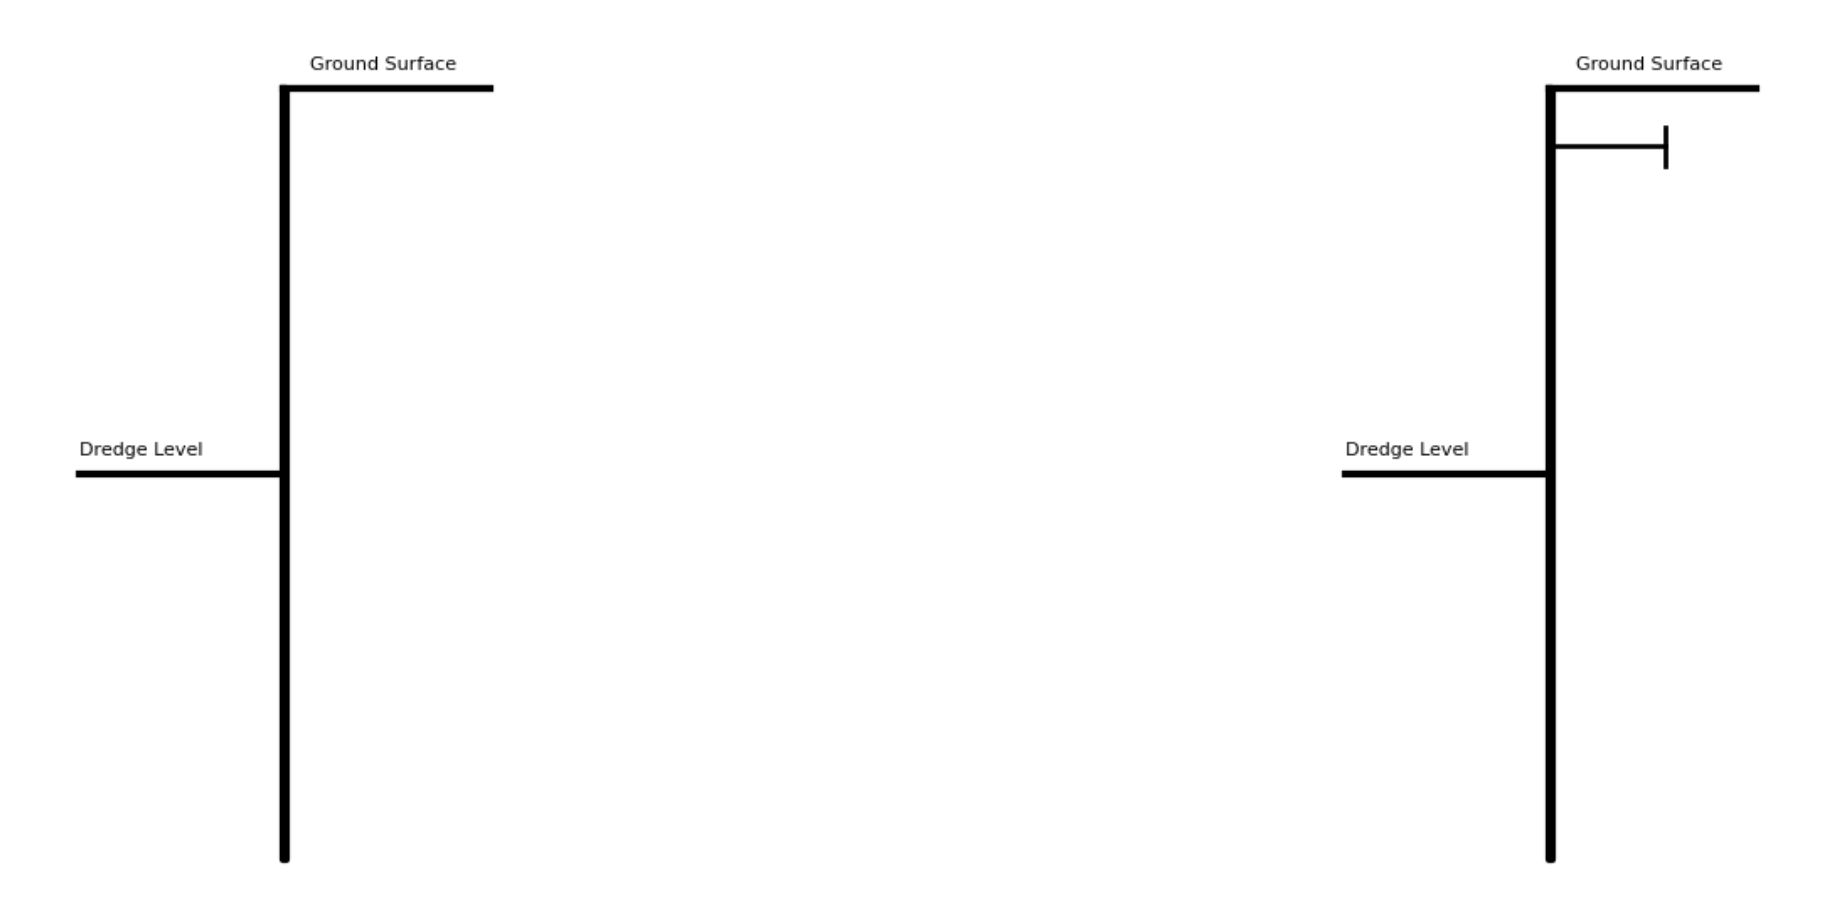
\includegraphics[width=0.75\linewidth]{figures/ch8/cantilever_anchored.png}
    \caption{Cantilever and anchored sheet pile wall}
    \label{fig:sheetpiles}
\end{figure}

Sheet pile walls can be made of multiple materials, like steel, concrete, or wood \autocite{brownDesignSheetPile1994}. For the design in this report, steel will be used as the advantages outweigh the disadvantages and are more suitable than concrete or wood. Concrete will have a longer service life, however, it will have higher initial costs compared to steel, and the installation of concrete walls is more difficult. Wooden walls can be used for shorter heights and temporary structures.  As discussed in Section \ref{section_8.2}, the advantages of steel sheet piles make it the most common material because of the strength, light weight, and long service life, in combination with the favorable ratio of cross-section and moment of resistance \autocite{brownDesignSheetPile1994}. The following section will outline the key steel properties relevant to the design.

The sections and interlocks for the steel sheet pile walls are crucial for completing a wall when  using it for waterfront structures \autocite{baxterPilingHandbook2022}. Figure \ref{fig:sections_sheetpiles} shows typical steel sections widely used and goes by the names of U and Z sections. In this figure, the interlocks, which give the sections their strength, can also be seen. The interlocks of the U sections are on the neutral axis, and the ones for the Z sections are not. In the neutral axis, the maximum shear stress is obtained, which means the interlocks should be welded or crimped to obtain the full moment of resistance \autocite{kellyMechanicsLectureNotes2018}. When sections meet with water, the walls must be watertight. This can be done with plastic compound materials filling the interlocks or using a preformed polyurethane interlock seal \autocite{baxterPilingHandbook2022}. 

\begin{figure}[H]
    \centering
    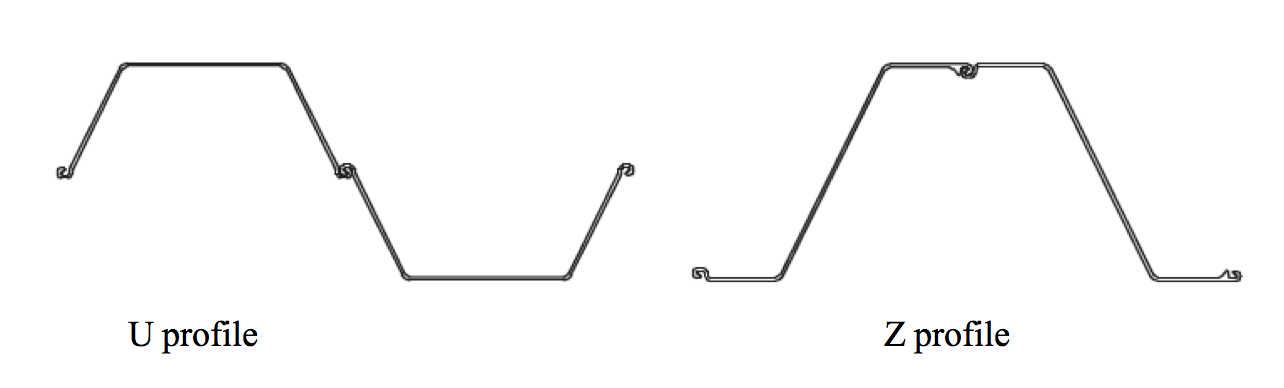
\includegraphics[width=0.50\linewidth]{figures/ch8/u_profile_z_profile.png}
    \caption{U and Z sections \autocite{sheetpilinggroupSheetPiles2018}}
    \label{fig:sections_sheetpiles}
\end{figure}

Steel will be the material used for the sheet piles. The properties of steel, as a homogeneous material, will be briefly introduced. Steel is an elastic material with a favourable strength-to-weight ratio and a tensile strength ranging between 300 and 2000 N/mm\textsuperscript{2} \autocite{grabeSheetPilingHandbook2008}. Beyond its general mechanical advantages, understanding the stress–strain behaviour of steel is essential for the design. The stress-strain behaviour of steel can be seen in Figure \ref{fig:stress_strain_steel}. The range of elasticity depends on the grade of steel, and the elastic modulus for steel, E, is  210000 N/mm\textsuperscript{2} \autocite{schipper81MaterialCharacteristics2024}. In Figure \ref{fig:stress_strain_steel}, f\textsubscript{y;d} is the design yield strength, which is the value where the stress will be constant, drop, or reach a strain of 0.2\% when the load is removed. Furthermore, f\textsubscript{t;d} is the design tensile strength, which is according to the grade of steel \autocite{grabeSheetPilingHandbook2008}. The mechanical properties of the steel used for the sheet piles are shown in Table \ref{tab:steel_materialproperties}.

\begin{figure}[H]
    \centering
    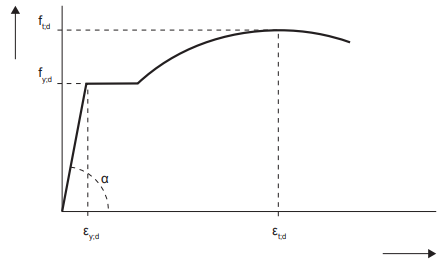
\includegraphics[width=0.70\linewidth]{figures/ch8/stress_strain_steel.png}
    \caption{Stress-strain relation steel \autocite{schipper81MaterialCharacteristics2024}}
    \label{fig:stress_strain_steel}
\end{figure}

\begin{table}[H]
  \centering
  \caption{Mechanical properties by steel grade \autocite{baxterPilingHandbook2022}}
  \label{tab:steel_materialproperties}
  \small
  \renewcommand{\arraystretch}{1.15}
  \begin{tabularx}{\linewidth}{@{}l l l l@{}}
    \toprule
    Steel grade &
    \makecell{Tensile strength $f_{u}\,[\mathrm{N/mm}^{2}]$} &
    \makecell{Yield strength $f_{y}\,[\mathrm{N/mm}^{2}]$} &
    \makecell{Elongation at failure $\varepsilon_{u}\,[\%]$} \\
    \midrule
    S 240 GP & 340 & 240 & 26 \\
    S 270 GP & 410 & 270 & 24 \\
    S 320 GP & 440 & 320 & 23 \\
    S 355 GP & 480 & 355 & 22 \\
    S 390 GP & 490 & 390 & 20 \\
    S 430 GP & 510 & 430 & 19 \\
    \bottomrule
  \end{tabularx}
\end{table}

Steel sheet piles are made of hot-rolled sections, which are made in the process of heating steel to temperatures of around 850 and 1200 $^{\circ}$C  above the recrystallization temperature before rolling \autocite{samarasekeraHotRolling2001}. This allows for the various shapes and larger sizes that are of importance with sheet piles. Compared with cold-rolled sections, hot-rolled sections generally have a slightly rougher surface and lower cost because additional cold-rolling and finishing processes are not required XX. A sustainable solution for sheet piles is found in the EPD ‘EcoSheetPiles™ Plus’ from ArcelorMittal. This steel sheet pile is produced by an electric arc furnace. In this process, 100\% renewable electricity and 100\% scrap steel are used for production \autocite{arcelormittalGuidelinesSustainabilitySteel2024}. Compared to the blast furnace, the production of CO\textsubscript{2} is significantly reduced. In this way a more sustainable solution is used as the conventional one.

% \subsubsection{Sustainability}

% In Table \ref{tab:env_impacts}, an overview of the materials, concrete, steel and timber is provided in relation to the emissions $CO_{2}$ and the energy consumption. As can be seen from the table, the production and use of steel is the least sustainable. However, the choice of steel is made based on the advantages of the profile and its fast installation. In this paragraph, research is conducted to assess which profile is most sustainable for the design of the steel sheet piles.

% \begin{table}[H]
%   \centering
%   \caption{Environmental impacts by material \autocite{schipper81MaterialCharacteristics}}
%   \label{tab:env_impacts}
%   \small
%   \setlength{\tabcolsep}{6pt}
%   \renewcommand{\arraystretch}{1.15}
%   \begin{tabularx}{\linewidth}{@{}l l l@{}}
%     \toprule
%     Material &
%     CO$_2$ emissions (kg CO$_2$e per ton) &
%     Energy consumption (MJ per ton) \\
%     \midrule
%     Concrete & 100 to 200 & 1200 to 1600 \\
%     Steel    & 1800 to 2000 & 20000 to 35000 \\
%     Timber   & -600 to -1200 & 500 to 1000 \\
%     \bottomrule
%   \end{tabularx}
% \end{table}

% A sustainable solution for sheet piles is found in the EPD ‘EcoSheetPiles™ Plus’ from ArcelorMittal. This steel sheet pile is produced by an electric arc furnace. In this process, $100\%$ renewable electricity and $100\%$ scrap steel are used for production \autocite{arcelormittalGuidelinesSustainabilitySteel2024}. Compared to the blast furnace, the production of $CO_{2}$ is significantly reduced, as can be seen in Figure \ref{fig:eaf_bof}. In this way a more sustainable solution is used as the conventional one.

% \begin{figure}[H]
%     \centering
%     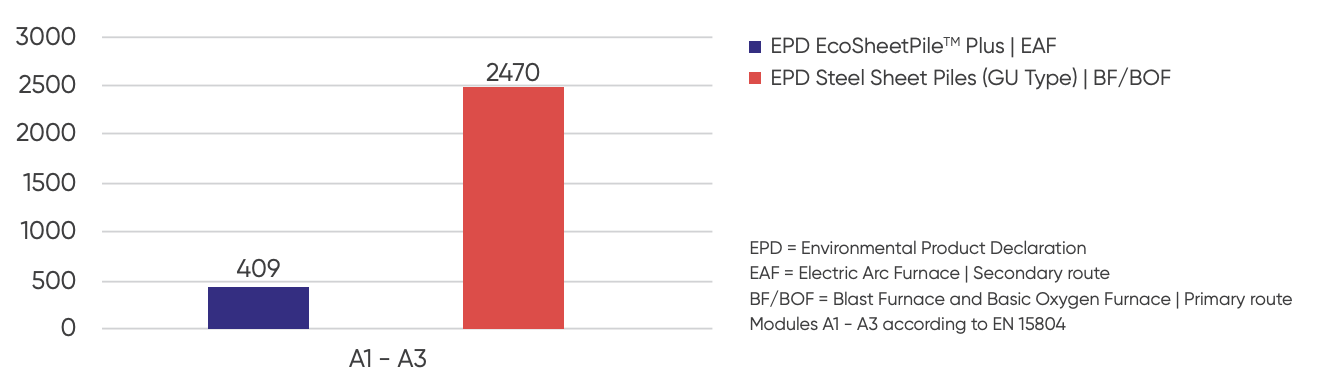
\includegraphics[width=0.90\linewidth]{figures/ch8/eaf_bof.png}
%     \caption{Global warming potential [kg CO2e/t sheet pil] \autocite{arcelormittalGuidelinesSustainabilitySteel2024}}
%     \label{fig:eaf_bof}
% \end{figure}

% NOG EVEN GOED UITZOEKEN NAAR WELKE MATERIAL PROPERTIES BELANGRIJK KUNNEN ZIJN. OOK EVEN SUSTAINABILITY IN ACHT NEMEN MET DE GEVONDEN DOCUMENTEN. WELLICHT EEN KOPJE SUSTAINABILITY EN WAT PLOTJES LATEN ZIEN.

\subsubsection{Failure mechanisms}

Sheet piles have failure mechanisms related to flexural, rotational, and deep seated failure. These failure mechanisms for cantilever sheet piles are shown in Figure \ref{fig:failure_mechanisms_sheetpiles} as told from left to right. Within the design of a sheet pile, these failure mechanisms have to be taken into account and verifications should be performed to check whether the failure mechanisms are arising.

The flexural failure mechanism shown on the left of Figure \ref{fig:failure_mechanisms_sheetpiles} shows that the cantilever pile is failing due to the bending moments exerted by the earth and the pressure of the water \autocite{brownDesignSheetPile1994}. This happens when the bending action on the wall is greater than the resistance of the chosen profile and exceeds the strength of the material. Rotating failure occurs when the sheet pile close to the base rotates about a pivot point \autocite{brownDesignSheetPile1994}. This happens because there is no balance between the lateral pressure of the earth, which results in a collapse, as shown in the center of Figure \ref{fig:failure_mechanisms_sheetpiles}. The final failure mechanism related to cantilever sheet piles is the deep seated failure. This failure mechanism occurs when the soil mass around the sheet pile rotates along a surface \autocite{brownDesignSheetPile1994}, which is shown on the right side of Figure \ref{fig:failure_mechanisms_sheetpiles}.

\begin{figure}[H]
    \centering
    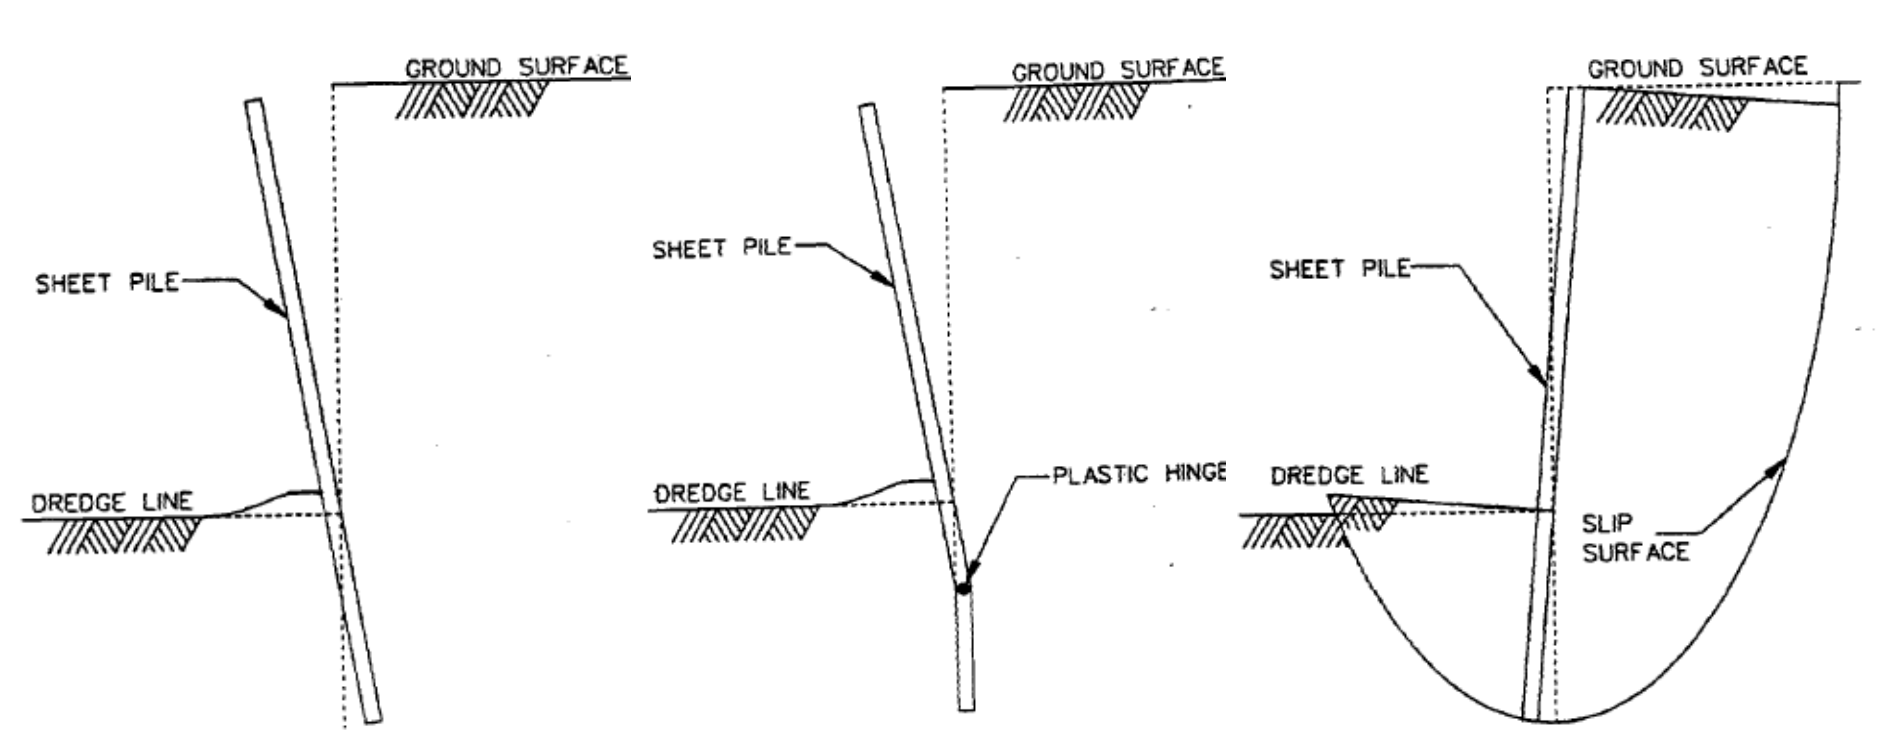
\includegraphics[width=0.90\linewidth]{figures/ch8/failure_mechanisms.png}
    \caption{Failure mechanisms cantilever sheet pile wall \autocite{brownDesignSheetPile1994}}
    \label{fig:failure_mechanisms_sheetpiles}
\end{figure}

% HIER NOG DE FAILURE MECHANISMS BESPREKEN. EVEN KIJKEN WAAROM IK HIER AL ALLEEN DE CANTILEVER LAAT ZIEN. WELLICHT OOK DIE VAN DE ANCHORED LATEN ZIEN OMDAT DE KEUZE PAS VERDER WORDT GEMAAKT.

\subsection{Geotechnical parameters}
\label{section:geotechnical_parameters}

For the design, the soil layers, including their geotechnical parameters, should be known. In Paragraph \ref{par:geology}, the geological background for the area of interest is explained, and this serves as the basis for deriving the soil layers and parameters. The borehole in Figure \ref{fig:borehole} is deemed the most relevant source. The borehole shows a top layer with fine/medium sands. Below, clay/clayey sand can be found, and the bottom layer consists of medium sand. This is in accordance with the geological profile that was provided before in Figure \ref{fig:geolprofile}, which describes a transition from near-surface beach ridges, dunes, beach plains, and delta sub-aerial facies to deeper open estuaries and marine deposists. The top deposits help declare the presence of sandy deposits at the top of the borehole and the layers of clay/clayey sand below correspond to estuarine deposits. Finally, old marine/fluvial deposits were likely compacted and lead to the layer of medium sand found at the bottom of the borehole.

Because of the resemblance between the local borehole and the geological profile given before, the layering as shown in Figure \ref{fig:borehole} is deemed representative for the whole study area. Based on this layering the relevant parameters can be derived, the result is shown in Table \ref{tab:soil_layers}. The parameters in Table \ref{tab:soil_layers} were derived from the Eurocode \autocite{stichtingkoninklijknederlandsnormalisatieinstituutNederlandseNormNEN2025}. Because of limited knowledge on soil characteristics, conservative estimates were made based on this code. In the borehole, no explicit information is given on the top fill layer. Therefore, conservative parameters were assumed based on typical values for organic topsoil. As derived from the borehole and the overview in Table \ref{tab:soil_layers}, the soil profile with the specific layers and properties is shown in Figure \ref{fig:soil_profile_cross_section}. 

\begin{table}[H]
  \centering
  \caption{Characteristic values soil}
  \label{tab:soil_layers}
  \small
  \setlength{\tabcolsep}{6pt}
  \renewcommand{\arraystretch}{1.15}
  \begin{tabularx}{\linewidth}{@{}p{1.6cm}l p{1.6cm}*{5}{Y}@{}}
    \toprule
    Layer &
    Soil type &
    Depth [m] &
    $\gamma_d\,[\mathrm{kN/m}^3]$ &
    $\gamma_{\!sat}\,[\mathrm{kN/m}^3]$ &
    $\varphi'\,[{}^\circ]$ &
    ${c'}\,[\mathrm{kPa}]$ &
    ${c_u}\,[\mathrm{kPa}]$ \\
    \midrule
    1 & Fill               & 0.0 - 2.0   & 12 & 12 & 15.0 & 2.5 & 20 \\
    2 & Fine/medium sand   & 2.0 - 7.0   & 17 & 19 & 30.0 & 0.0 & \textemdash \\
    3 & Clay               & 7.0 - 10.0  & 14 & 14 & 17.5 & 0.0 & 25 \\
    4 & Clayey sand        & 10.0 - 15.0 & 18 & 20 & 25.0 & 0.0 & \textemdash \\
    5 & Clay               & 15.0 - 16.0 & 14 & 14 & 17.5 & 0.0 & 25 \\
    6 & Clayey sand        & 16.0 - 17.5 & 18 & 20 & 25.0 & 0.0 & \textemdash \\
    7 & Medium sand        & 17.5 - 32.0 & 18 & 20 & 32.5 & 0.0 & \textemdash \\
    \bottomrule
  \end{tabularx}
\end{table}

% \begin{figure}[H]
%     \centering
%     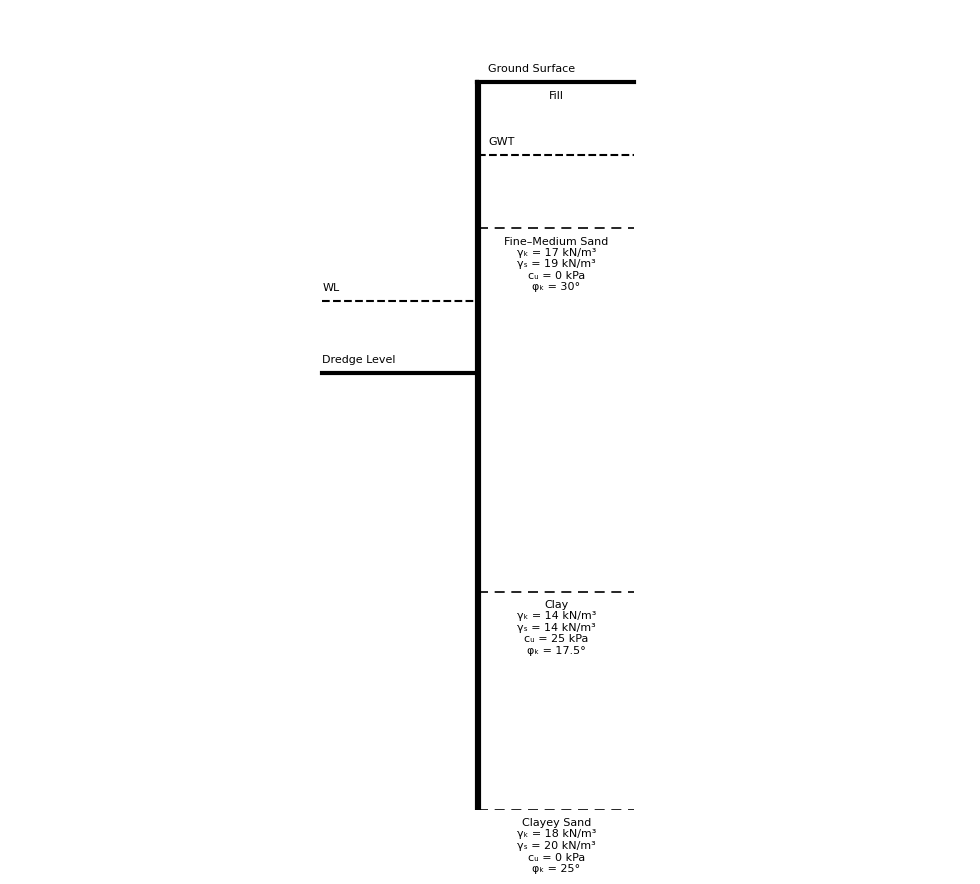
\includegraphics[width=0.90\linewidth]{figures/ch8/soil_profile.png}
%     \caption{Soil profile and properties}
%     \label{fig:soil_profile_cross_section}
% \end{figure}

\newpage

\subsection{Hydraulic parameters}
\label{section:hydraulic_parameters}

In addition to geotechnical parameters, the design of the cantilever sheet pile wall is also based on hydraulic parameters. In this design, the sheet pile wall is located in open water and has a groundwater table. Because of this, the hydrostatic pressure will act on both sides of the wall. The water level of the river and the groundwater may differ in level, and when this is the case, an excess of hydrostatic pressure will act on the sheet pile. 

In addition to this, the elevation of the water level is important. The design value of the water level is based on the levels on interpolated elevations in the water levels between Brazo Largo and Ibicuy. In Figure \ref{fig:water_levels_camping}, this time series of water elevations can be seen, in which a period of 4 years with time intervals of 20 minutes is used. As water levels fluctuate over the years and the lowest water level will be governing, the design water level is derived with the lower bound of the 95\% confidence interval. In this case the design water elevation determined to be equal to +0.14 m IGN. Using the water elevation of 25 September, the date of the field trip, the ground surface in relation to IGN can be derived. This will be done in the geometry of the problem in the following section. 

\begin{figure}[H]
    \centering
    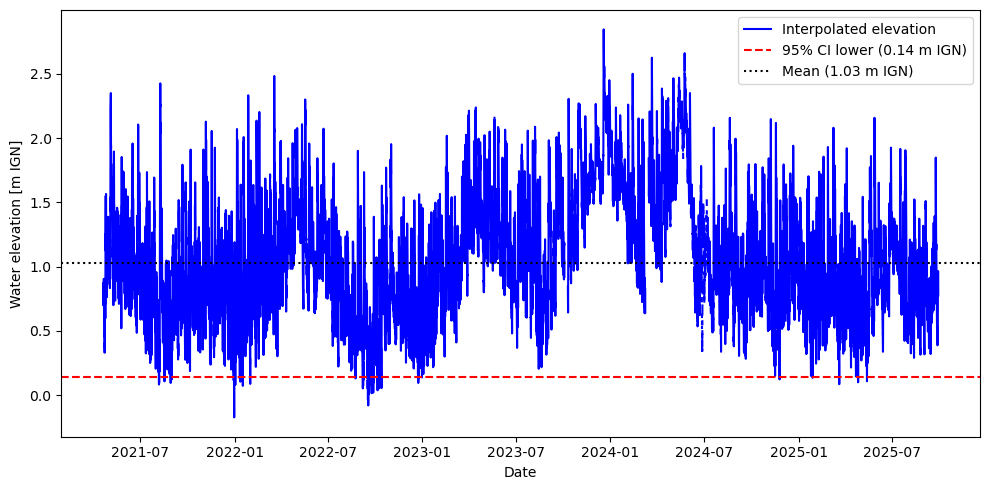
\includegraphics[width=0.60\linewidth]{figures/ch8/waterlevel_camping blanqueda.png}
    \caption{Water levels camping Blanqueda}
    \label{fig:water_levels_camping}
\end{figure}

To determine the level of the riverbed, the bathymetry of the location analysed in Section \ref{section:cirtical_location} is used. The theory of bathymetry is covered in Chapter \ref{chap:hydroanalysis}. In Figure \ref{fig:bath}, the bathymetry taken for this location can be seen and the corresponding development of the river bed can be seen in Figure \ref{fig:bath2}. In this figure, the vertical value near the river bank is -1.97 m IGN. Taking into account the distance between the bathymetry and the bank, a value of –1.5 m IGN is assumed at the bank, and this is adopted as the riverbed level.

\begin{figure}[H]
    \centering
    \begin{subfigure}{0.65\linewidth}
        \centering
        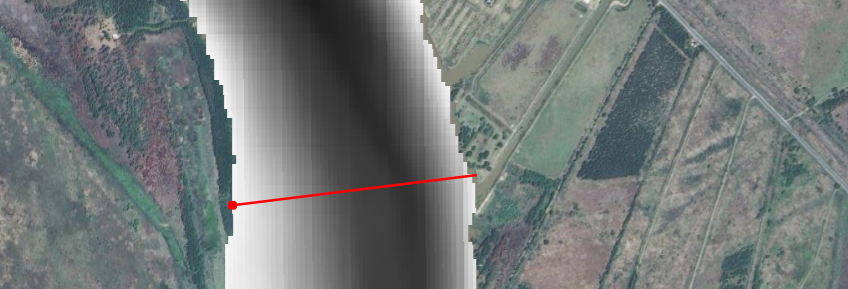
\includegraphics[width=\linewidth]{figures/ch8/bathemetry_1.png}
        \caption{Location of bathymetry}
        \label{fig:bath}
    \end{subfigure}

    \begin{subfigure}{0.65\linewidth}
        \centering
        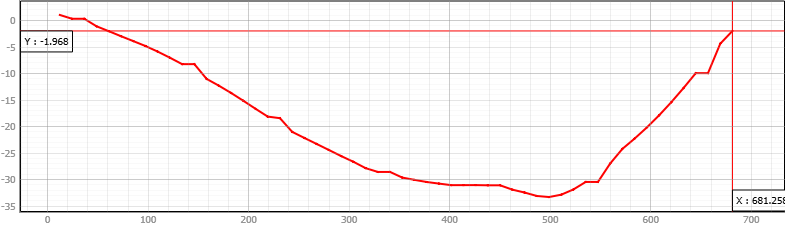
\includegraphics[width=\linewidth]{figures/ch8/bathemetry_2.png}
        \caption{Bathymetry riverbed cross-section}
        \label{fig:bath2}
    \end{subfigure}

    \caption{Bathymetry analysis}
    \label{fig:bath_combined}
\end{figure}


% AANNAMES

% RIVERBED OP -1.5M DOOR DE AFSTAND TUSSEN OEVER EN BATH. WATER LEVEL, GEINTERPOLEERDE METINGEN TUSSEN BRAZO LARGO EN IBICUY VAN ELEVATIONS. WATERLEVEL IS UITGEDRUKT IN ELEVATION EN DAT IS METER ING. DESIGN WATER LEVEL IS GEBASEERD OP 95% LOWER BOUND VAN DE CONFIDENCE INTERVAL. NEEM AAN OP BASIS VAN FOTO DAT HET HOOGTE VERSCHIL MINIMAAL EEN 1.0-1.5M, DUS DAAROM EEN DESIGN WAARDE VAN 2.5M IGN MAAIVELD. 

% KWA FIGUREN: BATHEMTRY PLUS CROSS-SECTION LOCATION. INFORMATIE OVER DE GEBRUIKTE BT STAAT IN SECTION 7.1.1. 

% TIMESERIES VAN WATER ELEVATIONS. HIERVAN ZEGGEN DAT HET HISTORISCHE DATA IS MET 20MIN INTERVAL VOOR DATA PUNTEN. OVER 4 JAAR.

\newpage

\subsection{Design of steel sheet pile}

The design of steel sheet piles begins with defining the design location and problem description to get a better understanding of the situation. After defining these conditions, a method is considered to calculate the earth pressure and water pressure. These pressures are then used to balance the moments and iteratively define the embedding depth of the sheet pile wall. After calculating the embedding depth based on the balance of moments, the sheet pile is verified according to structural verifications, including bending moments, shear force, and deflection.  

To set up the balance of moments for defining the embedding depth, the loads acting on the wall need to be defined. The lateral loads acting on the wall include soil and water pressure, which need to be defined to calculate the forces. The soil parameters are defined, and the soil profile is taken from Section \ref{section:geotechnical_parameters}. With the soil profile and its parameters, the earth pressures can be defined on both sides of the sheet pile wall. The hydraulic pressure due to the water levels is of importance, and these are defined in Section \ref{section:hydraulic_parameters}. 

With the problem description defined, a plan to calculate the embedding depth of the sheet pile is set up by using Python code. The plan begins by defining the soil and water parameters, which will be transformed to effective stresses, active and passive earth, and hydrostatic water pressures. From the stresses, the resulting forces acting on the sheet pile wall are defined, and a balance of moments is obtained. Setting the moment to zero at the bottom of the sheet pile wall, the embedding depth is calculated iteratively.

The determination of the critical erosion points along the river has been done in Section \ref{section:cirtical_location}. The location analysed here will be the location for which the design of the steel sheet pile will be based. In Figure \ref{fig:critical_location_google}, the critical point is shown in Aqua Monitor, and during the field trip, images were taken to verify if erosion was visible. The total length is 215 meters, which is drawn and shown in Table \ref{tab:Surface Lost Camping La Blanqueada in 2022}.

\begin{figure}[H]
    \centering
    \begin{subfigure}[b]{0.45\textwidth}
        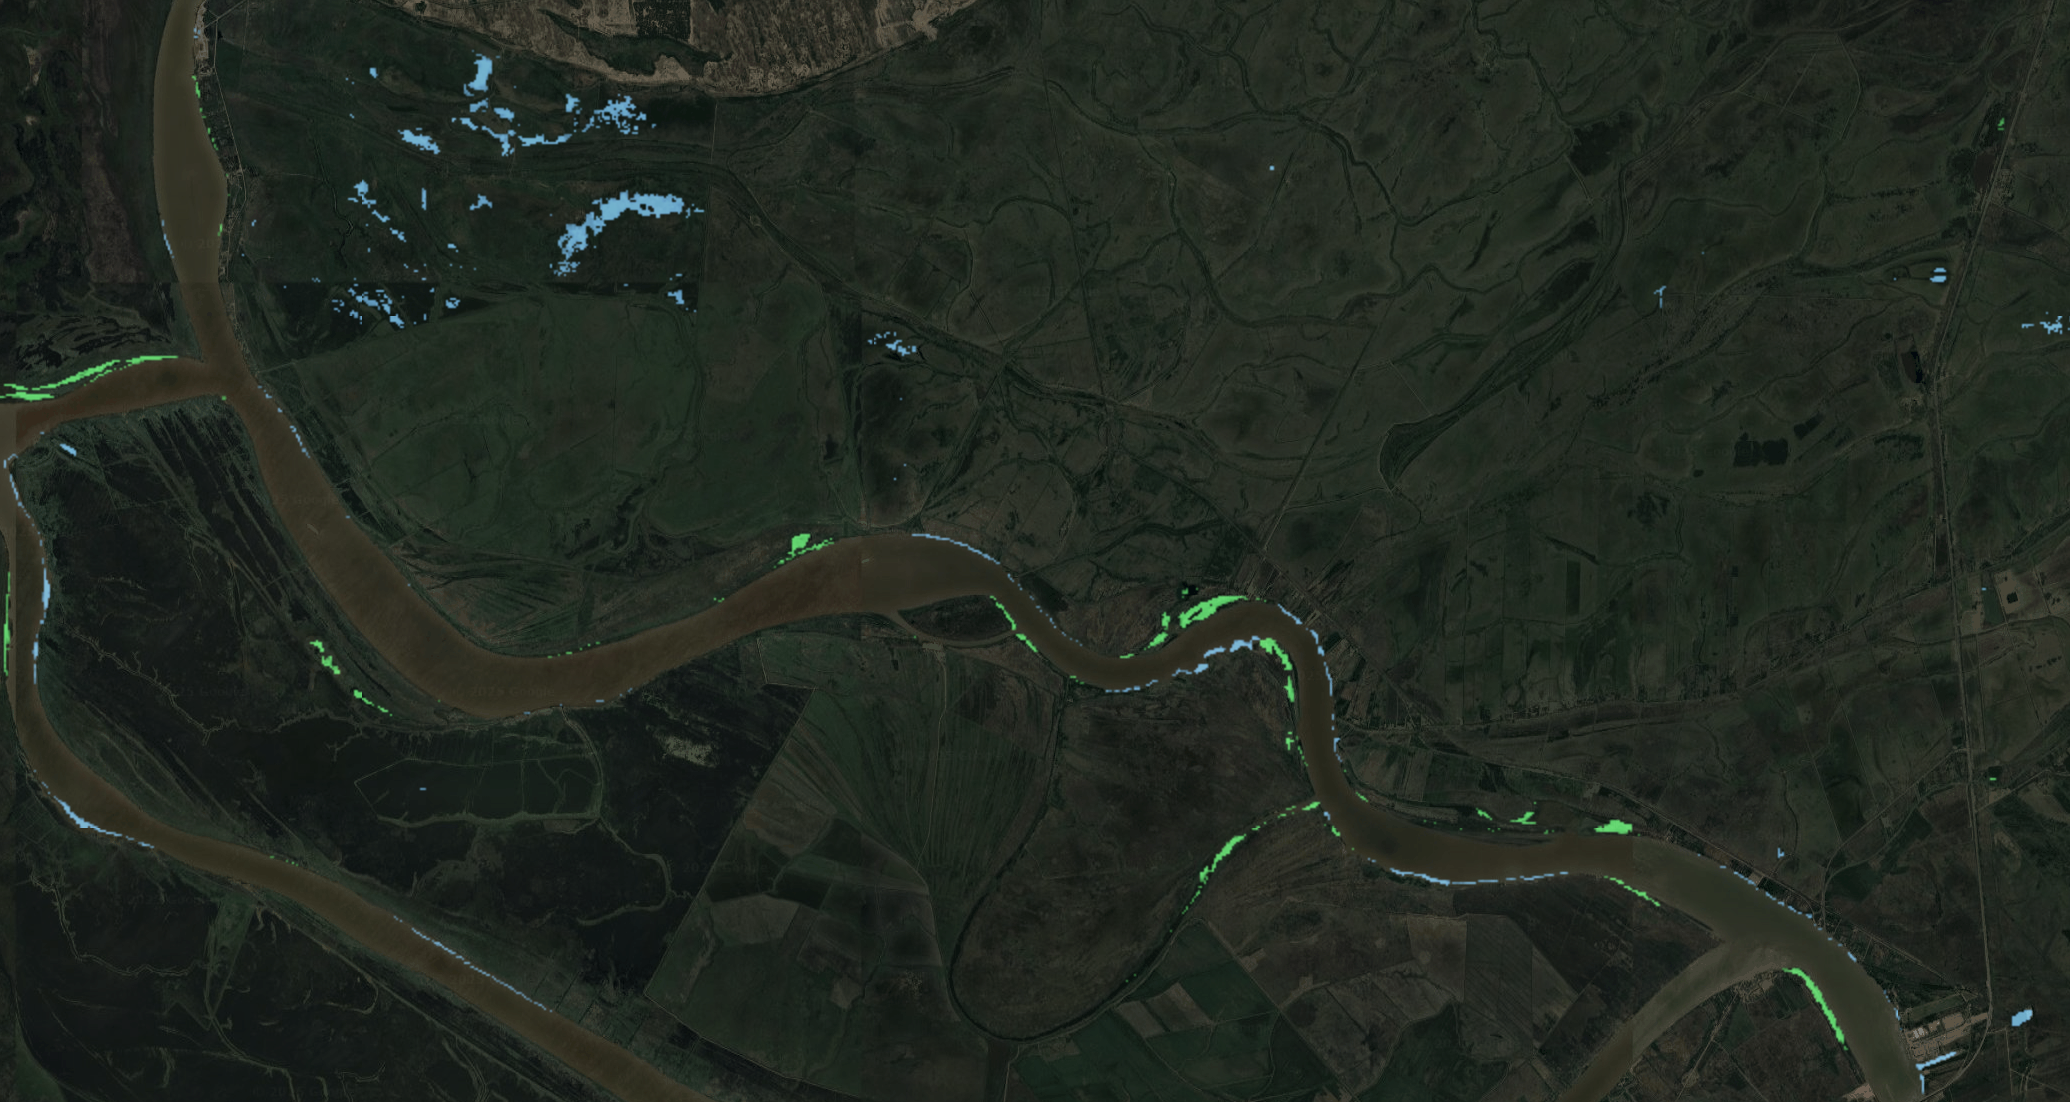
\includegraphics[width=\linewidth, height=5cm]{figures/ch8/critical_location_google.png}
        \caption{Critical location Aqua Monitor}
        \label{fig:critical_location_google}
    \end{subfigure}
    \hfill
    \begin{subfigure}[b]{0.45\textwidth}
        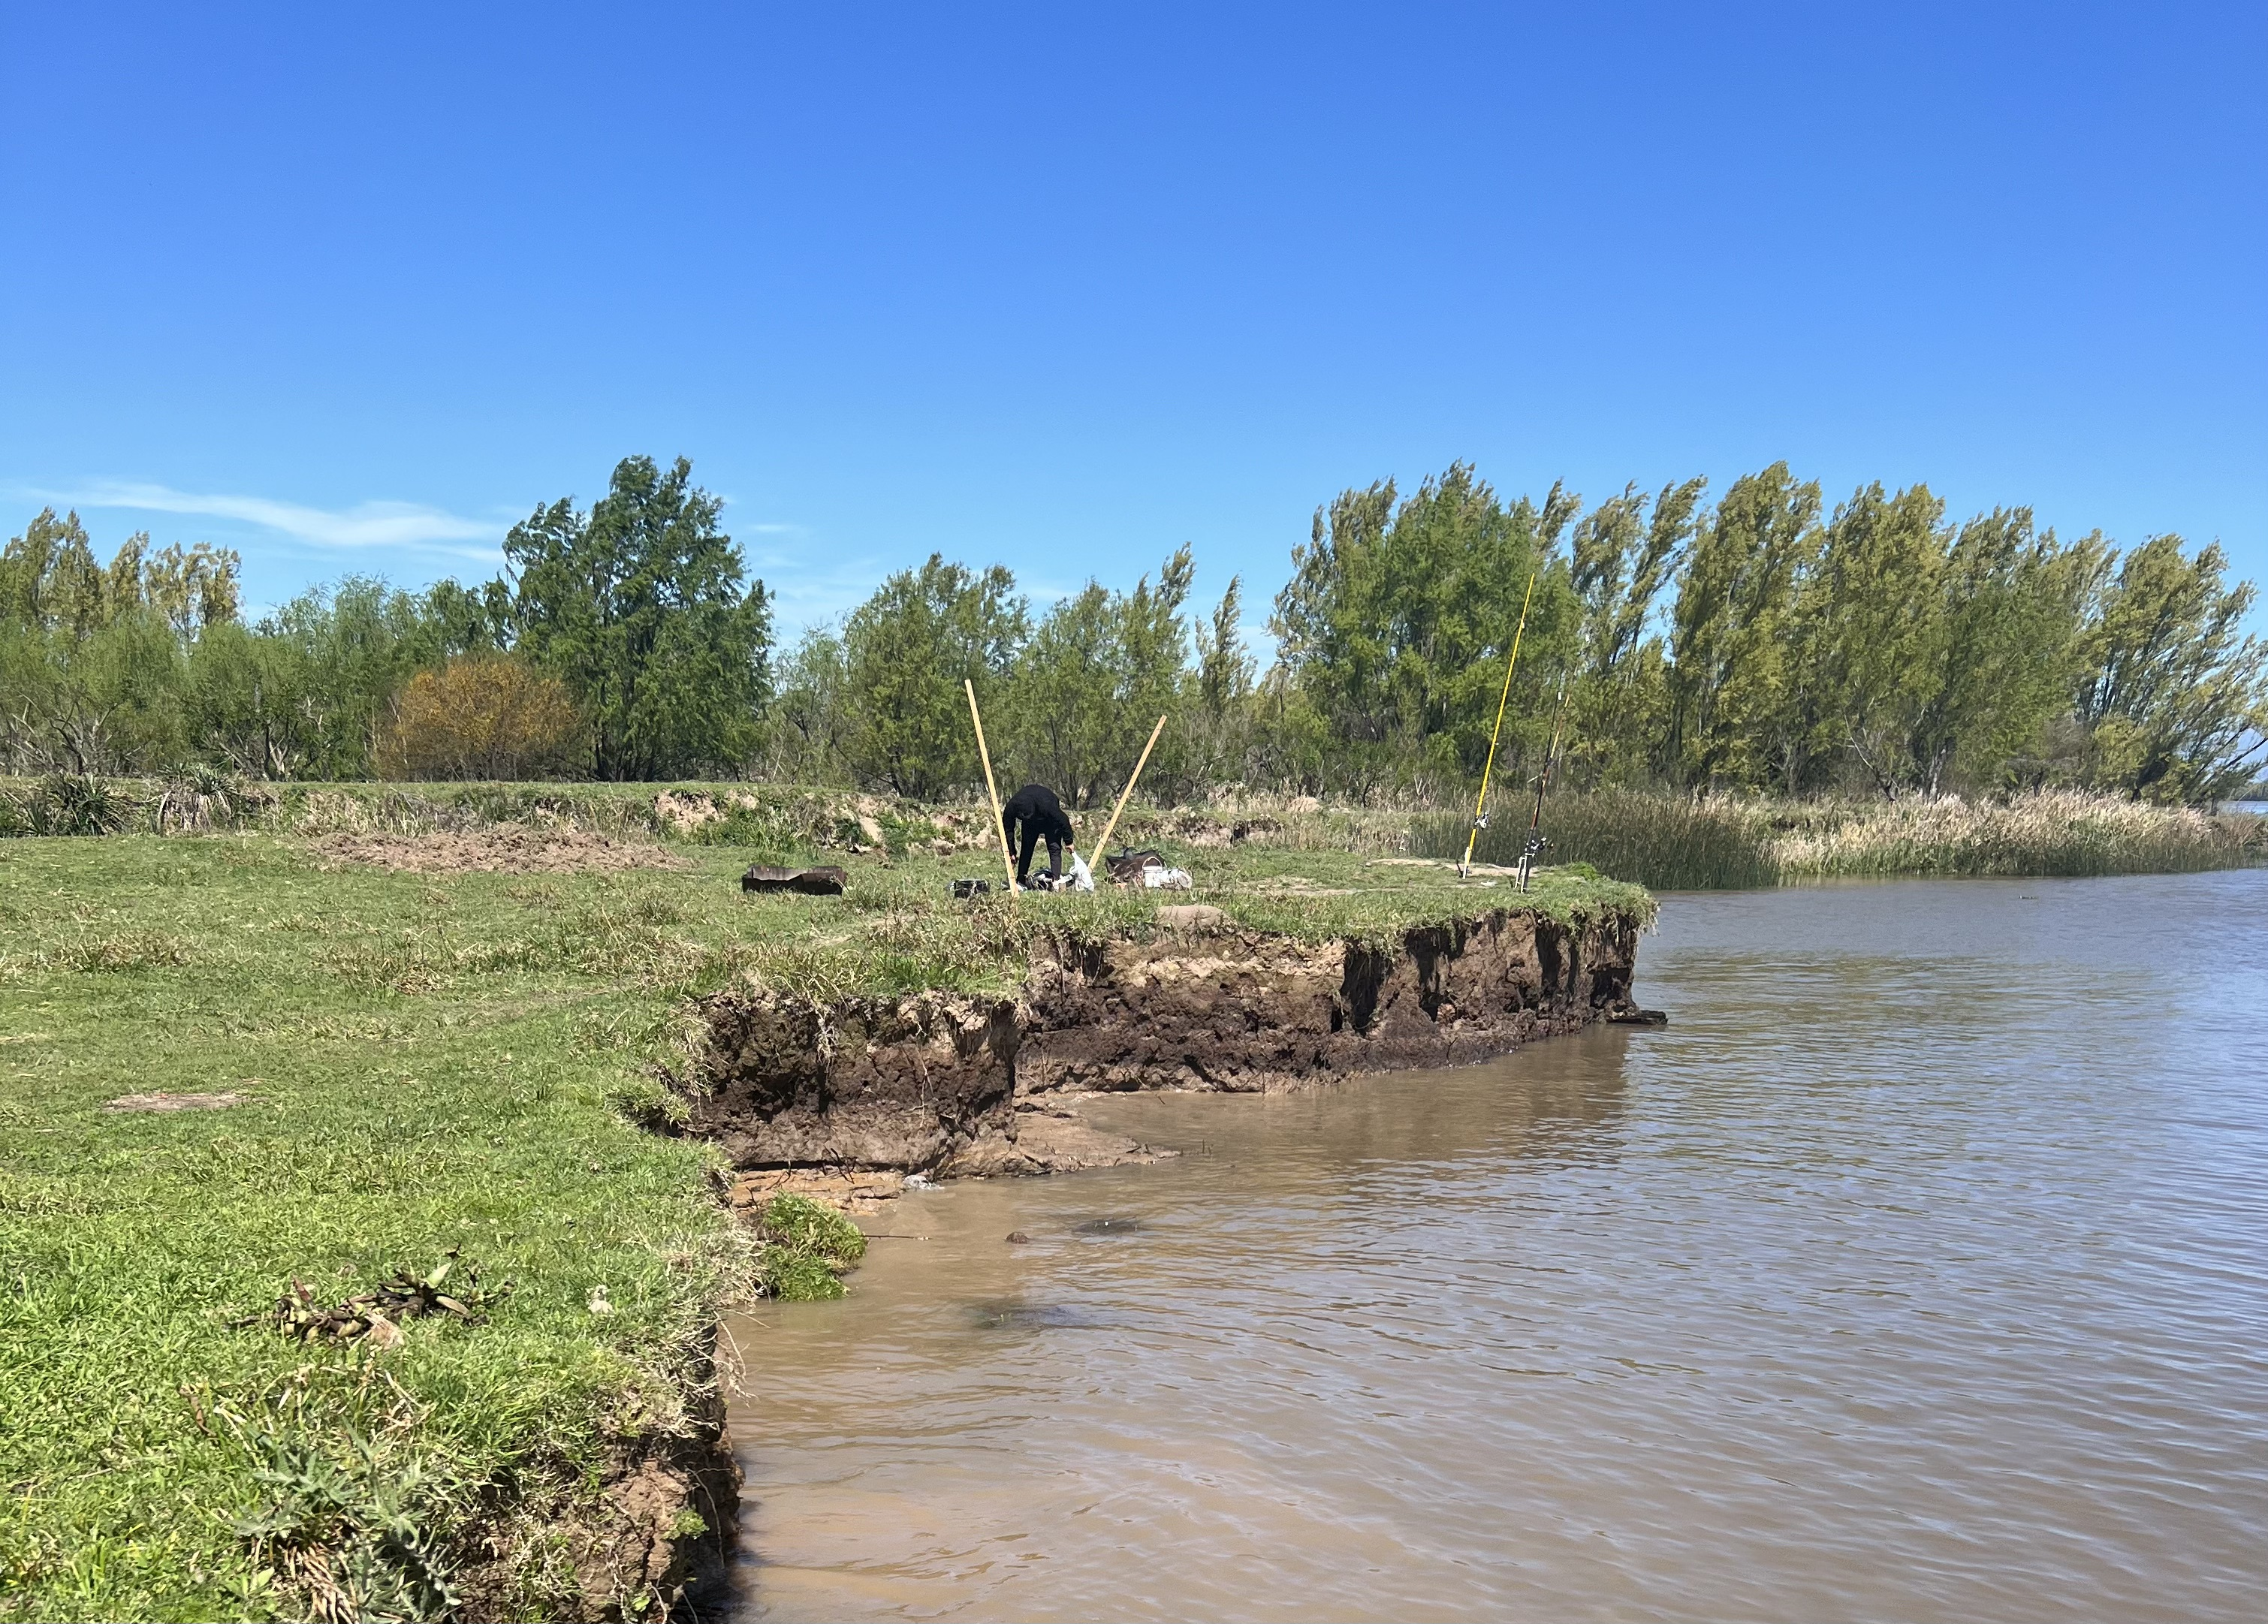
\includegraphics[width=\linewidth, height=5cm]{figures/ch8/critical_location.jpeg}
        \caption{Verification critical point field trip}
        \label{fig:critical_location_fieldtrip}
    \end{subfigure}
    \caption{Design location for steel sheet pile}
    \label{fig:critical_location}
\end{figure}

\subsubsection{Geometry of the problem}

The design of the sheet pile wall is based on the cantilever sheet pile wall. As briefly touched on in Section \ref{section:sheet_pile_wall}, the cantilever sheet pile is used to maintain heights up to $5$ meters and is supported by the soil and hydrostatic pressure. In Figure \ref{fig:problem_description_sheetpiles}, a sketch of the situation is provided, which is written in Python. The height that must be retained, $4.0$ meters, is indicated by $Z$. The embedding depth of the cantilever sheet pile, which will need to be determined iteratively, is noted as $t$. In  Section \ref{section:hydraulic_parameters}, the levels of the groundwater table, the water level and the dredge level are derived. The water level of the river is indicated as $WL$, which in this situation is $+0.14$ meters. The dredge level is $-1.5$ meters. The groundwater table is $+1.03$ meters, indicated as $GWT$. The ground surface is derived from comparing the water elevation on 25 September 14:00:00 from the time series, with Figure \ref{fig:critical_location_fieldtrip}. The ground surface level is assumed to be $1.5$ meters higher than the time series value of $1.0$ meters, resulting in $+2.5$ m IGN.

\begin{figure}[H]
    \centering
    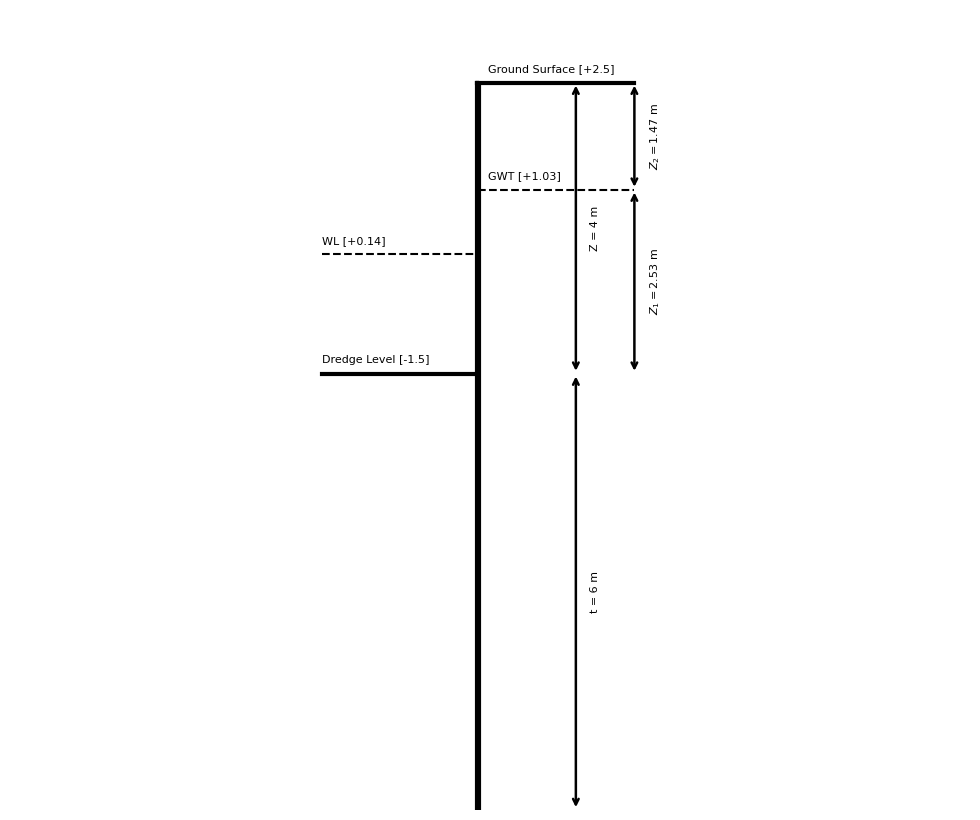
\includegraphics[width=1.0\linewidth]{figures/ch8/cross_section.png}
    \caption{Cross-section for sheet pile}
    \label{fig:problem_description_sheetpiles}
\end{figure}

% \begin{itemize}
%     \item WL is the water level;
%     \item GWT is the ground water table;
%     \item Z is the retained height;
%     \item t is the embedding depth;
%     \item $Z_{1}$ is the unsaturated soil height;
%     \item $Z_{2}$ is the saturated soil height.
% \end{itemize}

\subsubsection{Method}

The design of a cantilever sheet pile can be performed using multiple classical design methods or numerical analysis. Common approaches applicable to sheet pile walls include the methods of Bishop, Homberg, Padfield, and Mair, Bowles, Day, and Das, as well as the free earth method, the spring-supported beam method, and numerical models such as PLAXIS FEM.

Reviewing Eurocode 7, the calculation for the design of a sheet pile should be based on the spring-supported beam method \autocite{eurocodeGeotechnicalDesignStructures2025}. However, due to complexity, the sheet pile wall will be calculated using the simplified Padfield and Mair method. This method is a simplified representation of the situation, however, after calculating the embedding depth, the verifications will be according to the ultimate limit and serviceability limit defined in Eurocode 3 and Eurocode 7.

% \subsubsection{Simplified Padfield and Mair}

The simplified Padfield and Mair method XX used for the cantilever sheet pile is a simplified graphical method, shown in Figure \ref{fig:blum}. The right side of the sheet pile is the active side, and the left side, below the dredge level, is the passive side. The simplification step in the figure shows an additional resultant force, R, which acts on the lowest point of the sheet pile. This is done because below this point the active and passive sides switch, creating a complex situation. Within the method, plastic development of the soil and water table level is assumed to be infinitely stiff. All the support is obtained by the fixity of the soil. To calculate the embedding depth, the sum of moments around the lowest fixed point "O" of the sheet pile wall will be set to zero. The unknown embedding depth can be calculated in multiple ways. In this section, an initial embedding depth will be defined, and iteratively, the moment will be set to zero while increasing or decreasing the embedding depth. However, in this method, no safety factors are taken into account. Therefore, the embedding depth must be increased by 20\%.

\begin{figure}[H]
    \centering
    \begin{subfigure}[b]{0.35\textwidth}
        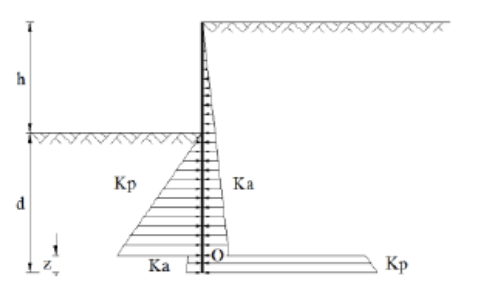
\includegraphics[width=\linewidth, height=5cm]{figures/ch8/blum_1.png}
        \caption{Full method}
        \label{fig:conventional_design}
    \end{subfigure}
    \begin{subfigure}[b]{0.35\textwidth}
        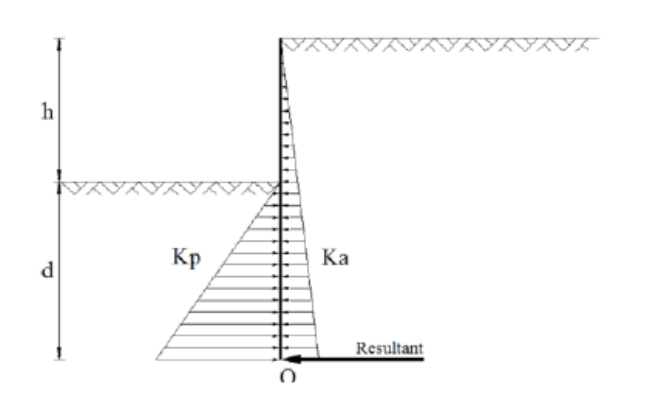
\includegraphics[width=\linewidth, height=5cm]{figures/ch8/blum_2.png}
        \caption{Simplified method}
        \label{fig:blum_simplification}
    \end{subfigure}
    \caption{Simplified method Padfield and Mair XX}
    \label{fig:blum}
\end{figure}

\subsection{Calculation of the embedding depth}
\label{section:embedding_depth}

The embedding depth of the sheet pile is derived from the balance of moment around the lowest point. The balance of moments should be set to zero, providing the minimal embedding depth. To make up the balance of moments, the pressures acting on the sheet pile should be defined to transform these into forces. The horizontal pressure acting on the sheet pile is the earth and hydrostatic pressure. First, the earth pressures are analysed in Python code. Hereafter, the hydrostatic analysis will be performed, and the forces will be calculated. 

The depth can be defined in multiple ways. A method is to keep the depth as an unknown parameter, t. This provides an explicit formula for moving below the dredge line, for the pressure and resulting forces. As the forces will be related to the balance of moments, roots are obtained to get the unknown t. However, another approach is to begin with an estimated depth and calculate the sum of moments around the lowest point. As this balance will not be zero, an iterative solution can be used to make sure the depth is increasing while optimizing the moment balance to zero at the lowest part of the sheet pile. In this design, the depth of the sheet pile is based on the second approach. The first value of the embedding depth is taken as 6.0 meters, which can be seen in Figure \ref{fig:problem_description_sheetpiles}.

\subsubsection{Effective stress}

The horizontal pressure of the soil can be calculated based on the effective stress. The effective stress in the soil can be calculated with Equation \ref{eq:effective_stress}. The stress is based on the height of the soil and the unit weight $\gamma$ of each layer. If the soil layer is below the groundwater table, the saturated unit weight should be deducted from the unit weight, $\gamma - \gamma_{w}$. In Figure \ref{eq:effective_stress}, the effective stress on both sides of the sheet pile can be seen, and the corresponding values are provided in Table \ref{tab:appendix_effective_stress}.

\begin{equation}
    \sigma^{'}_{z} = z \cdot \gamma
    \label{eq:effective_stress}
\end{equation}

\begin{figure}[H]
    \centering
    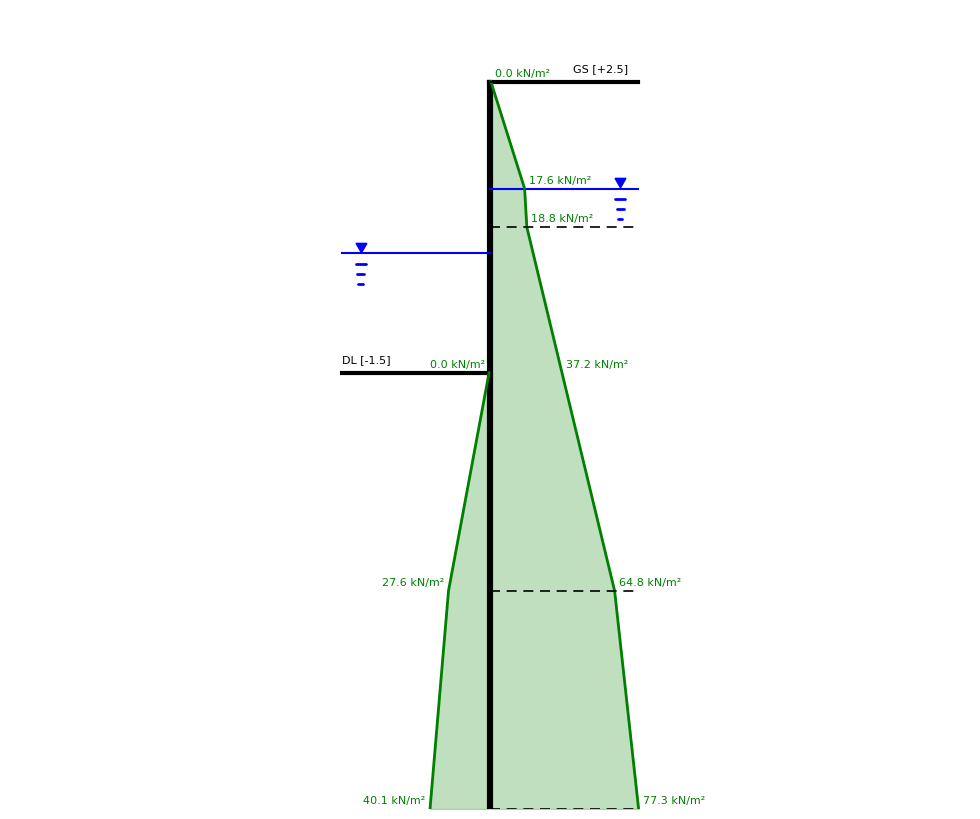
\includegraphics[width=0.7\linewidth]{figures/ch8/effective_stress.png}
    \caption{Effective stress active and passive side}
    \label{fig:effective_stress}
\end{figure}

\subsubsection{Earth pressure and force}

The pressure the wall feels from the soil is the lateral earth pressure. This earth pressure can be calculated with the effective vertical stress and a coefficient. While soil is largely dependent on nature, the stresses differ, just like the vertical effective stress along the profile. Equation \ref{eq:earth_pressure} shows how the earth pressures are calculated for both the active and passive sides. For the active and passive sides, the coefficients K\textseubscript{a} and \textseubscript{a} will be used.

\begin{equation}
    p_{ea,h,z} = z \cdot \gamma \cdot K_{\gamma}
    \label{eq:earth_pressure}
\end{equation}

The active and passive earth coefficients can be computed by Equations \ref{eq:K_gamma_a_k} and \ref{eq:K_gamma_p_k}. These equations are regarding the Coulomb theory and in this calculation the $\alpha$, $\beta$, and $\delta$, which are the slope of the sheet pile, slope of the ground levels, and wall friction angle are equal to zero \autocite{grabeSheetPilingHandbook2008}. Therefore, Equations \ref{eq:Ka_tan} and \ref{eq:Kp_tan} are used.

\begin{equation}
    K_{\gamma;a;k} =
    \frac{
        \cos^{2}\!\left(\varphi' + \alpha\right)
    }{
        \cos^{2}(\alpha)
        \left(
            1 +
            \sqrt{
                \frac{
                    \sin\!\left(\varphi' + \delta_{a;k}\right)
                    \sin\!\left(\varphi' - \beta_a\right)
                }{
                    \cos\!\left(\alpha - \delta_{a;k}\right)
                    \cos\!\left(\alpha + \beta_a\right)
                }
            }
        \right)^{2}
    }
    \label{eq:K_gamma_a_k}
\end{equation}

\begin{equation}
    K_{\gamma;p;k} =
    \frac{
        \cos^{2}\!\left(\varphi' - \alpha\right)
    }{
        \cos^{2}(\alpha)
        \left(
            1 -
            \sqrt{
                \frac{
                    \sin\!\left(\varphi' - \delta_{p;rep}\right)
                    \sin\!\left(\varphi' + \beta_p\right)
                }{
                    \cos\!\left(\alpha - \delta_{p;k}\right)
                    \cos\!\left(\alpha + \beta_p\right)
                }
            }
        \right)^{2}
    }
    \label{eq:K_gamma_p_k}
\end{equation}

\begin{equation}
    K_{\gamma,a} = \tan^{2}\!\left(45^\circ - \frac{\varphi'}{2}\right)
    \label{eq:Ka_tan}
\end{equation}

\begin{equation}
    K_{\gamma,p} = \tan^{2}\!\left(45^\circ + \frac{\varphi'}{2}\right)
    \label{eq:Kp_tan}
\end{equation}

Using Table \ref{tab:soil_layers}, in which all soil parameters are included, the effective angle of internal friction is needed to calculate the active and passive coefficients for the different layers. Table \ref{tab:layers_ka_kp} gives an overview of the active and passive coefficients for the different layers. 

\begin{table}[H]
  \centering
  \caption{Soil layers and earth pressure coefficients.}
  \label{tab:layers_ka_kp}
  \small
  \setlength{\tabcolsep}{8pt}
  \renewcommand{\arraystretch}{1.15}
  \begin{tabular}{@{}r l l r r r@{}}
    \toprule
    Layer & Soil type & Depth [m] &
    $\varphi'\,[\boldsymbol{^\circ}]$ &
    $K_{\gamma,a}$ [-] & $K_{\gamma,p}$ [-] \\
    \midrule
    1 & Fill             & 0.0 - 2.0   & 15.0 & 0.589 & - \\
    2 & Fine--Medium Sand& 2.0 - 7.0   & 30.0 & 0.333 & 3.000 \\
    3 & Clay             & 7.0 - 10.0  & 17.5 & 0.538 & 1.860 \\
    4 & Clayey Sand      & 10.0 - 15.0 & 25.0 & 0.406 & 2.464 \\
    \bottomrule 
  \end{tabular}
\end{table}

Figure \ref{fig:earth_pressure} shows an overview of the active and passive earth pressure acting on the wall. These values are shown in Appendix \ref{appendix:earth_pressure}. When calculating the earth pressures, it should be noted that for the interfaces of the soil layers, the rightful coefficient is taken and multiplied with the effective stress, $\sigma_{z}$. From the active and passive pressure acting on the sheet pile, one can determine the horizontal forces. The horizontal force is calculated with Equation \ref{eq:earth_force} within Python, where the active and passive earth pressure is multiplied by the height of its layer. For triangular shapes, the Equation \ref{eq:earth_force} should be multiplied by a factor of $\frac{1}{2}$.

For the force magnitude, triangles and rectangles were computed by Python, and the corresponding forces were defined. In Figure \ref{fig:earth_pressure}, an overview of all the forces is shown. An overview of the segments, corresponding values, and point of application is shown in Table \ref{tab:appendix_forces_centroids}.

\begin{equation}
    F_{ea,h,z} = p_{ea,h,z} \cdot h_{layer}
    \label{eq:earth_force}
\end{equation}

\begin{figure}[H]
    \centering
    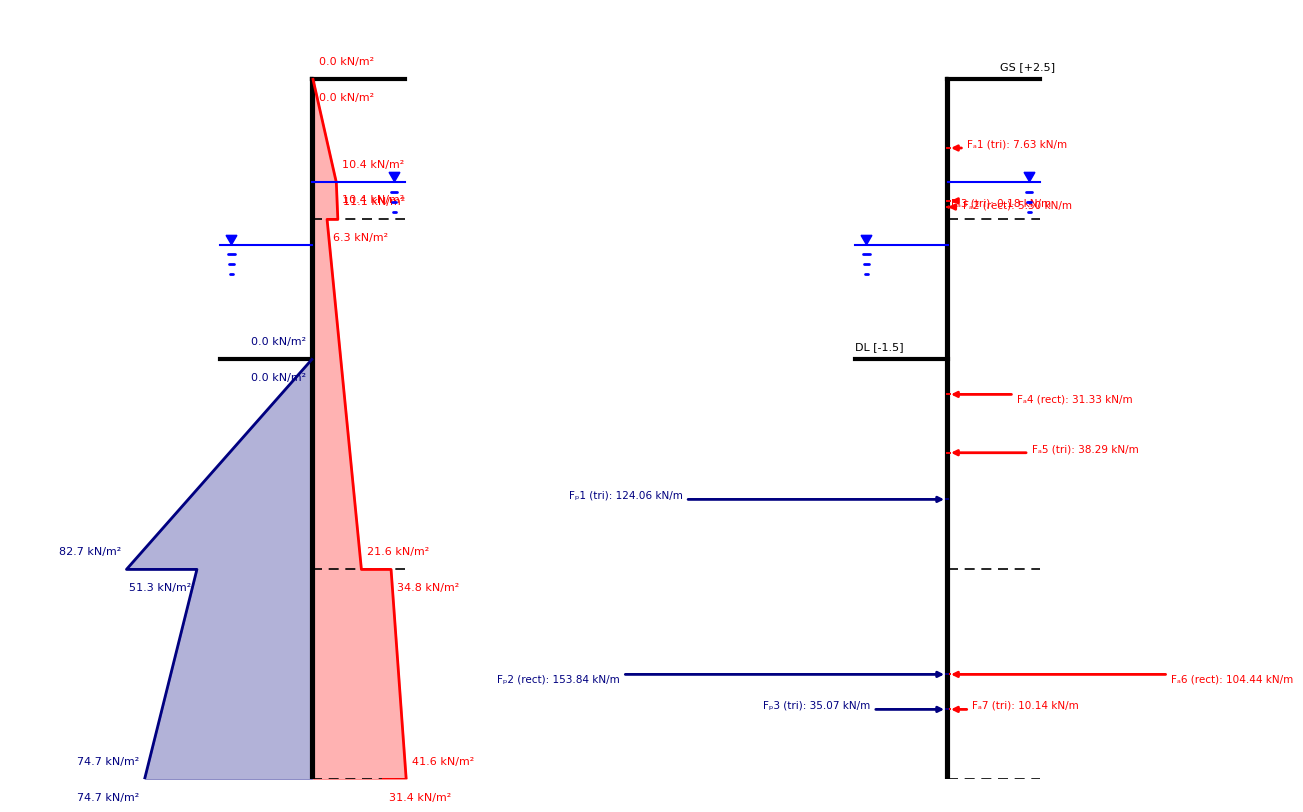
\includegraphics[width=0.75\linewidth]{figures/ch8/earth_pressure_force.png}
    \caption{Earth pressure active/passive side (left) and resulting force (right)}
    \label{fig:earth_pressure}
\end{figure}

\newpage

\subsubsection{Hydrostatic pressure and force}

The hydrostatic pressure $w$ is referred to as the pore water pressure \autocite{grabeSheetPilingHandbook2008}. In unconfined groundwater, the pore water pressure at a depth z is calculated by Equation \ref{eq:pore_water_pressure}.

\begin{equation}
    w = z \cdot \gamma_{w}
    \label{eq:pore_water_pressure}
\end{equation}

When there is an excess of hydrostatic pressure, meaning that the water levels on both sides of the wall are not at the same level, an excess hydrostatic pressure will occur. The excess hydrostatic pressure can be calculated with Equation \ref{eq:excess_water_pressure}. In Figure \ref{fig:hydrostatic_excess_pressure}, an overview of the hydrostatic water pressure and force is given. The corresponding values are shown in Table \ref{tab:appenidx_u_profile}. 

\begin{equation}
    w_{u}(z) = w_{r}(z) - w_{l}(z) = h_{r}(z) \cdot \gamma_{w} - h_{l}(z) \cdot \gamma_{w}
    \label{eq:excess_water_pressure}
\end{equation}

\begin{figure}[H]
    \centering
    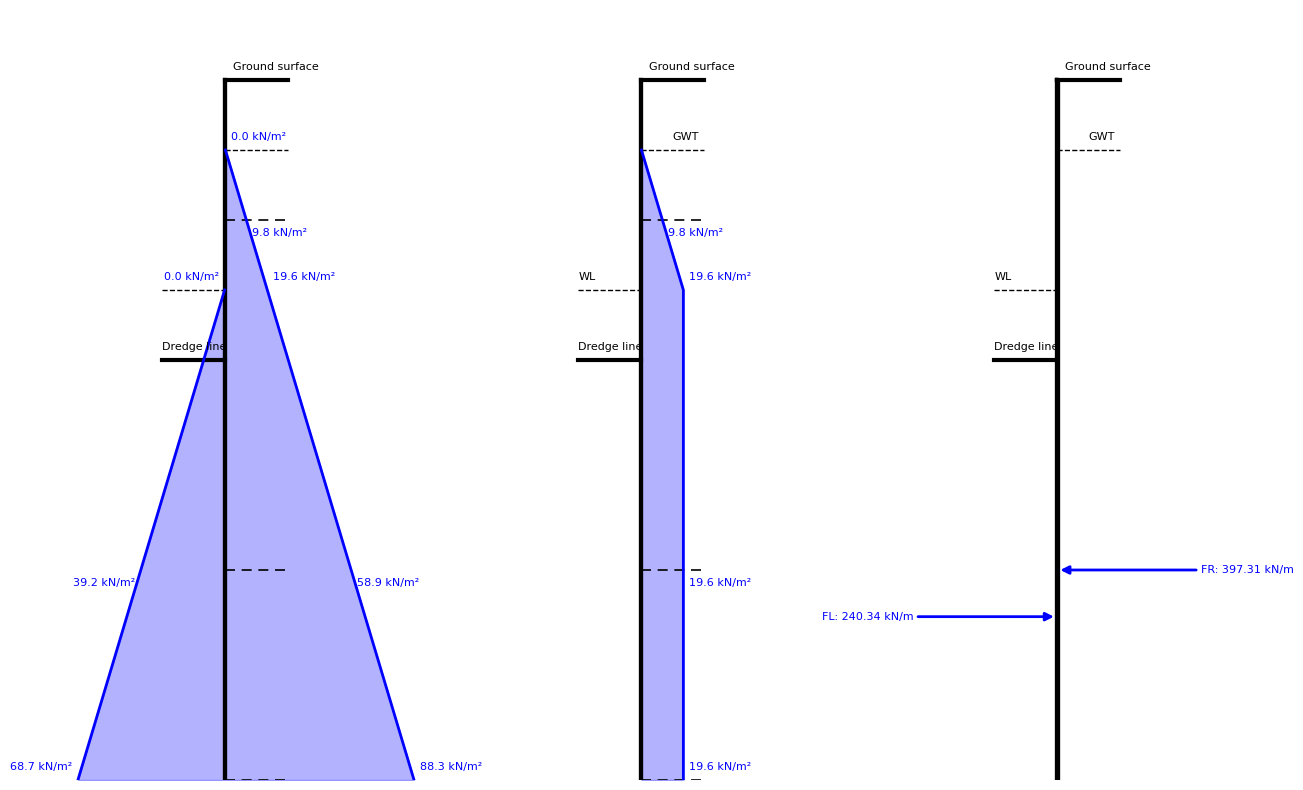
\includegraphics[width=0.75\linewidth]{figures/ch8/water_overview.png}
    \caption{Hydrostatic pressure (left), excess hydrostatic pressure (center), and forces (right)}
    \label{fig:hydrostatic_excess_pressure}
\end{figure}

\subsubsection{Bending moment}

The balance of moments around the lowest part of the sheet pile should be zero,  stated in Equation \ref{eq:moment}. For $t = 6.0$ meters, in Figure \ref{fig:appendix_moments_balance_6000}, this point, "O", is indicated, and the forces acting due to both the earth and hydrostatic pressure are shown. From the acting forces and the distance to point "O", the moments are computed. In Table \ref{tab:appendix_forces_arms_moments_now}, it can be seen that the balance of moments, for t = 6.0 meters, is not equal to zero, but 156.3 kNm/m. Indicating an iterative calculation, increasing the embedding depth, and checking at which depth the moments are equal to zero, is required.

\begin{equation}
    \sum{M_{t}} = 0
    \label{eq:moment}
\end{equation}

 After an iteration process, in Python, the embedding depth is set to 7.574 meters. In Figure \ref{fig:appendix_moments_balance_6000}, the forces related to this depth are shown. In Table \ref{tab:forces_arms_moments_9713}, the values of the forces and moments are shown, and the resulting moment around the point "O" is close to zero, 0.0512 kNm/m. Regarding the safety factor, the simplified Padfield and Mair method says that the depth of embedding found should be increased by 20\%, giving the following depth:

\begin{equation}
    t_{simplified} = 1.20 \cdot 7.574 = 9.09 \ m
\end{equation}

\begin{figure}[H]
    \centering
    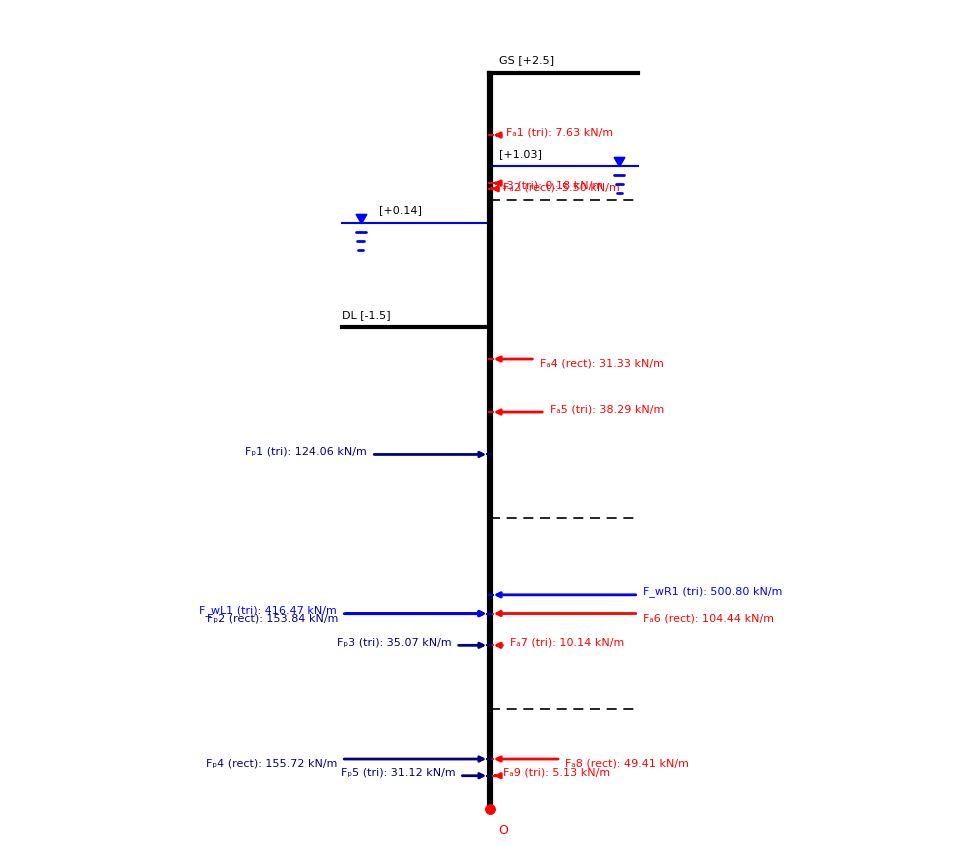
\includegraphics[width=0.90\linewidth]{figures/ch8/moment_balance_7574.png}
    \caption{Forces for t = 7.574 meters}
    \label{fig:final_moments_balance}
\end{figure}

\begin{table}[H]
  \centering
  \caption{Resultant forces, arms, and moments for t = 7.574 meters}
  \label{tab:forces_arms_moments_9713}
  \small
  \setlength{\tabcolsep}{8pt}
  \renewcommand{\arraystretch}{1.15}
  \begin{tabular}{@{}l l r r r@{}}
    \toprule
    Side & Shape &
    F [kN/m] & $z_{base}$ [m] &
    $M_{\text{base}}$ [kN$\cdot$m/m] \\
    \midrule
    Active  & Triangle  &   7.63  & 10.59 &  80.88 \\
    Active  & Rectangle &   5.50  &  9.84 &  54.16 \\
    Active  & Triangle  &   0.18  &  9.75 &   1.77 \\
    Active  & Rectangle &  31.33  &  7.07 & 221.67 \\
    Active  & Triangle  &  38.29  &  6.24 & 238.98 \\
    Active  & Rectangle & 104.44  &  3.07 & 321.08 \\
    Active  & Triangle  &  10.14  &  2.57 &  26.10 \\
    Active  & Rectangle &  49.41  &  0.79 &  38.90 \\
    Active  & Triangle  &   5.13  &  0.52 &   2.69 \\
    Hydro passive   & Triangle  & 416.47  &  3.07 & -1279.17 \\
    Hydro active    & Triangle  & 500.80  &  3.37 & 1686.78 \\
    Passive & Triangle  & 124.06  &  5.57 &  -691.60 \\
    Passive & Rectangle & 153.84  &  3.07 &  -472.98 \\
    Passive & Triangle  &  35.07  &  2.57 &   -90.29 \\
    Passive & Rectangle & 155.72  &  0.79 &  -122.59 \\
    Passive & Triangle  &  31.12  &  0.52 &   -16.33 \\
    \midrule
    $\sum M_{t}$ (should ≈ 0 for equilibrium) & & & & 0.0512 \\
    \bottomrule
  \end{tabular}
\end{table}

\subsection{Ultimate Limit State GEO}

A cantilever sheet pile wall should be designed according to two conditions. These conditions are the Ultimate Limit State (ULS) and the Serviceability Limit State (SLS). In the ULS, the worst possible forces that can occur during the span of the sheet pile should be analyzed with respect to the safety of people and the structure \autocite{baxterPilingHandbook2022}. In the SLS checking the structure under normal conditions where the function and appearance of the structure are concerned \autocite{baxterPilingHandbook2022}. In this section, the ULS GEO is performed.

For the design, this means that safety factors for the ULS and SLS should be included, regarding Eurocode 7 GEO \autocite{stichtingkoninklijknederlandsnormalisatieinstituutNederlandseNormNEN2025}, which is not included in the simplified Padfield and Mair method. For the analysis, multiple combinations should be verified, and the most unfavourable is used for the design. Two combinations, within design approach 1, stated in Eurocode 7, are evaluated in Appendix \ref{appendix:uls_combinations}. However, for the calculation in this section, the most unfavourable combination is taken and elaborated.

The most unfavourable combination within design approach 1 is combination 2 (DA1-2). The safety factors are shown in Table \ref{tab:partial_factors}, and the partial factors on loads, materials, and actions to protect the sheet pile in ULS are shown \autocite{stichtingkoninklijknederlandsnormalisatieinstituutNederlandseNormNEN2025}. In this calculation, the hydrostatic loads and the earth pressures are permanent. For SLS, all safety factors are set at $1.0$. The combination and safety factors result in the final embedding depth of t = 10.172 meters,  shown in Figure \ref{fig:appendix_uls_moments_balance_forces}. However, the acting shear forces and bending moments are greater. From Table \ref{tab:appendix_forces_arms_moments_new}, it can be seen that the balance of moments at this depth is close to zero (-0.0632 kNm/m).

\begin{equation}
    t_{GEO} = 10.172 \ m
\end{equation}

\begin{table}[H]
\centering
\small
\setlength{\tabcolsep}{8pt}
\renewcommand{\arraystretch}{1.2}
\begin{tabular}{@{}l l l c c@{}}
\toprule
\multicolumn{1}{l}{Parameter} & 
\multicolumn{1}{l}{ } & 
\multicolumn{1}{l}{Partial factor} & 
\multicolumn{2}{c}{Combination}\\
\cmidrule(lr){4-5}
 & & & 1 & 2 \\
\midrule
\multirow{4}{*}{\textit{Actions}} 
 & Permanent, Unfavourable & $\gamma_G$ & 1.35 & 1.00 \\
 & Permanent, Favourable   & $\gamma_{G,\mathrm{fav}}$ & 1.00 & 1.00 \\
 & Variable, Unfavourable  & $\gamma_Q$ & 1.50 & 1.30 \\
 & Variable, Favourable\textsuperscript{1)} & -- & 0 & 0 \\
\midrule
\multirow{5}{*}{\textit{Material properties}} 
 & Effective shearing resistance & $\gamma_\varphi$ & 1.00 & 1.25 \\
 & Effective cohesion & $\gamma_c$ & 1.00 & 1.25 \\
 & Undrained shear strength & $\gamma_{cu}$ & 1.00 & 1.40 \\
 & Unconfined compressive strength & $\gamma_{qu}$ & 1.00 & 1.40 \\
 & Weight density & $\gamma_\gamma$ & 1.00 & 1.00 \\
\midrule
\textit{Earth resistance} & & $\gamma_{Re}$ & 1.00 & 1.00 \\
\bottomrule
\end{tabular}
\caption{Partial factors for actions, material properties, and earth resistance.}
\label{tab:partial_factors}
\end{table}

In Table \ref{tab:uls_summary}, an overview of the ULS analysis is shown. From this overview, it can be seen that the ULS combination DA1-2 is governing, and in the following section, these moments and shear will be verified with respect to the chosen profile. The bending moment lines are shown in Figures \ref{fig:appendix_bending_moments_DA1_1} and \ref{fig:appendix_bending_moments_DA1_1}. The shear lines are shown in Figures \ref{fig:appendix_shear_forces_DA1_1} and \ref{fig:appendix_shear_forces_DA1_2}.

\begin{table}[H]
  \centering
  \caption{Overview ULS combinations DA1-1 and DA1-2}
  \label{tab:uls_summary}
  \small
  \setlength{\tabcolsep}{8pt}
  \renewcommand{\arraystretch}{1.15}
  \begin{tabular}{@{}l r r r r r@{}}
    \toprule
    ULS & \multicolumn{1}{c}{Retained height [m]} & \multicolumn{1}{c}{Embedding depth [m]} & \multicolumn{1}{c}{Toe depth [m]} & \multicolumn{1}{c}{Max moment [kNm/m]} & \multicolumn{1}{c}{Max shear [kN/m]} \\
    \midrule
    DA1-1   & 4.0 & 7.58 & 11.6 & 280.5 & 220.6 \\
    DA1-2  & 4.0 & 10.17 & 14.2 & 404.4 & 266.6 \\
    \bottomrule
  \end{tabular}
\end{table}

\newpage

\subsection{Structural Verification ULS}
\label{section:structural_verification_uls}

In this structural verification of the cantilever sheet pile, a profile should be chosen and internally verified according to Eurocode \autocite{eurocodeEurocode3Design2007}. To perform the verifications, the section of the sheet pile should first be classified. Then verifications concerning the bending, shear, and combined bending and shear can be performed. In these verifications, the basic procedure for analyzing the profile will be that the actions do not exceed the resistance of the profile, shown in Equation \ref{limit_state}.

\begin{equation}
    E_{d} \leq R_{d}
    \label{limit_state}
\end{equation}

\begin{itemize}
    \item $E_{d}$ is design effects of actions;
    \item $R_{d}$ is design resistance.
\end{itemize}

In this section, the cross section AZ 24-700 from ArcelorMittal is verified \autocite{baxterPilingHandbook2022}. As this section will be placed in the river and is assumed to have fresh water, a corrosion factor should be incorporated. This means that the properties of the cross-section after corrosion will have a loss of thickness. From Eurocode 3, the total thickness loss, for a design working life of t\textsubscript{DWL} = 50 years, is calculated as follows:

\begin{equation}
    \Delta_{t} = \Delta_{tfront} +  \Delta_{tback} = 0.9 + 0.6 = 1.5 \ mm 
\end{equation}

With a loss of thickness of 1.5 millimetres, the properties regarding height, flange thickness, web thickness, sectional area, elastic section modulus, and plastic section modulus will be reduced. The reduced properties after erosion of this section are shown in Table \ref{tab:pu32}.

% Z PROFILES ARE STRONGER AND FOR WATER USE, DEEPER EXCAVATION

\begin{table}[H]
  \centering
  \small
  \setlength{\tabcolsep}{6pt}
  \renewcommand{\arraystretch}{1.15}
  \caption{Geometrical and mechanical properties of sheet pile section AZ 24-700 \autocite{baxterPilingHandbook2022}} 
  \label{tab:pu32}
  \begin{tabular}{@{}l l l c@{}}
    \toprule
    Property & Symbol & Units & AZ 24-700 \\
    \midrule
    Overall width                & $b$     & mm     & 700   \\
    Overall height               & $h$     & mm     & 457.5   \\
    Flange thickness             & $t_f$   & mm     & 9.7  \\
    Web thickness                & $t_w$   & mm     & 9.7  \\
    Flange breadth               & $b_f$   & mm     & 361   \\
    Slant angle                  & $\alpha$ & $^\circ$ & 55.2 \\
    Sectional area               & $A$     & cm$^2$/m & 163 \\
    Elastic section modulus      & $W_{el}$ & cm$^3$/m & 2435 \\
    Plastic section modulus      & $W_{pl}$ & cm$^3$/m & 2810 \\
    Moment of inertia            & $I$     & cm$^4$/m & 55890 \\
    Mass                         & ---     & kg/m$^2$ & 128 \\
    Class    & ---     & ---     & 3 \\
    \bottomrule
  \end{tabular}
\end{table}

\subsubsection{Section classification}

The classification of the steel profile tells whether the profile is behaving elastic or plastic. This is of importance when further analyzing the stability of the cantilever sheet pill with the bending and shear checks. The cross-section is classified by the flange slenderness ratio of the section. In Table \ref{tab:section_classification}, the classes and the ratios for Z and U profiles is shown. Formula \ref{eq:epsilon} is related to the coefficient that depends on the steel grade. 

\begin{equation}
    \epsilon = \sqrt{\frac{235}{f_{y}}}
    \label{eq:epsilon}
\end{equation}

\begin{itemize}
    \item $f_{y}$ is the yield strength [N/mm\textsuperscript{2}]
\end{itemize}

\begin{table}[H]
  \centering
  \small
  \setlength{\tabcolsep}{8pt}
  \renewcommand{\arraystretch}{1.15}
  \caption{Section classification}
  \label{tab:section_classification}
  \begin{tabular}{@{}l l c c@{}}
    \toprule
    \multicolumn{1}{l}{Class} &
    \multicolumn{1}{l}{Rotation check} &
    \multicolumn{2}{c}{Ratio of $b/t_f$ is less or equal than\ldots} \\
    \cmidrule(lr){3-4}
    & & Z-profile & U-profile \\
    \midrule
    \textit{1} & Required     & $45\,\varepsilon$ & $37\,\varepsilon$ \\
    \textit{2} & Not required & ---               & ---               \\
    \textit{3} & Not required & $66\,\varepsilon$ & $49\,\varepsilon$ \\
    \bottomrule
  \end{tabular}
\end{table}

For cross-section verification, the profile AZ 24-700 with the cross-section properties of Table \ref{tab:pu32} in grade S355 GP is classified as Class 3, with respect to Equation \ref{eq:class}. Therefore, no additional rotation check should be performed.

\begin{equation}
    \frac{b}{t_{f}} = \frac{361}{9.7} = 37.2 \leq 66 \epsilon 
    \label{eq:class}
\end{equation}

\subsubsection{Bending}

For the verification of bending, it is important that the design bending moment, M\textsubscript{Ed}, is smaller than the bending resistance, M\textsubscript{Rd}, of the profile. The maximum bending moment, M\textsubscript{Ed}, acting at the point of zero shear is 404.4 kNm/m, shown in Figure \ref{fig:appendix_bending_moments_DA1_2}. Within Class 3, Equation \ref{eq:bending_plastic} is used to calculate the bending resistance.

\begin{equation}
    M_{Ed} \leq M_{c,Rd}
\end{equation}

\begin{equation}
    M_{c,Rd} = \frac{\beta_{B} \cdot W_{el} \cdot f_{y}}{\gamma_{M0}}
    \label{eq:bending_plastic}
\end{equation}

\begin{itemize}
  \item $\beta_B$ is a factor that accounts for possible lack of shear force transmission in the interlocks between adjacent [-];
  \item $W_{el}$ is the cross-section’s elastic section modulus [cm\textsuperscript{3}/m];
  \item $f_y$ is the yield strength of steel [N/mm\textsuperscript{2}];
  \item $\gamma_{M0}$ is a partial factor [-].
\end{itemize}

Following the equation above, the bending moment resistance of the cross-section is calculated and verified with the following equations:

\begin{equation}
    M_{c,Rd} = \frac{1.00 \cdot 2430 \cdot 355}{1.0} = 862.7 \ kNm/m
\end{equation}

\begin{equation}
    \frac{M_{Ed}}{M_{Rd}} = \frac{404.4}{862.7} = 0.47
\end{equation}

\subsubsection{Shear}

For shear verification, it is important that the design shear force, V\textsubscript{Ed} is smaller than the plastic shear resistance, V\textsubscript{pl,Rd}, of the profile. The maximum shear force, V\textsubscript{Ed}, is 266.6 kN/m, shown in Figure \ref{fig:appendix_shear_forces_DA1_2}. Equation \ref{eq:shear_verification} is used to calculate the shear force resistance.

\begin{equation}
    V_{Ed} \leq V_{pl,Rd}
    \label{eq:shear_plastic}
\end{equation}

\begin{equation}
    V_{pl,Rd} = \frac{A_v \cdot f_{y}}{\sqrt{3} \cdot \gamma_{M0}}
    \label{eq:shear_verification}
\end{equation}

\begin{itemize}
    \item $A_{v}$ is the projected shear area of each web [mm\textsuperscript{2}];
    \item $t_w$ is the web’s thickness [mm];
    \item $t_f$ the flange thickness [mm];
    \item $h$ the overall height of the cross-section [mm].
\end{itemize}

Following the equation above, the shear force resistance of the cross-section is calculated and verified with the following equations:

\begin{equation}
    A_v = 9.7 \cdot (457.5 - 9.7) = 4343.7 \ mm^2
\end{equation}

\begin{equation}
    V_{pl,Rd} = \frac{4343.7 \cdot 355}{\sqrt{3} \cdot 1.0 \cdot 10^3} = 890.4 \ kN 
\end{equation}

\begin{equation}
    V'_{pl,Rd} = \frac{890.4}{0.7} = 1272 \ kN/m 
\end{equation}

\begin{equation}
    \frac{V_{Ed}}{V_{pl,Rd}} = \frac{266.6}{1272} = 0.21 
\end{equation}

\subsubsection{Combined bending and shear}

For the verification of the combinations of bending and shear, Equation \ref{eq:combi_shear_bending} should be satisfied. However, when the cross-section is classified as plastic, the effects of shear on plastic bending resistance can be neglected if Equation \ref{eq:combi_2_shear_bending} is satisfied. 

\begin{equation}
    M_{Ed} \leq M_{V,Rd} \ , \ M_{V,Rd} \leq M_{c,Rd}
    \label{eq:combi_shear_bending}
\end{equation}

\begin{equation}
    V_{Ed} \leq \frac{V_{pl,Rd}}{2}
    \label{eq:combi_2_shear_bending}
\end{equation}

\begin{itemize}
  \item $V_{Ed}$ is the design shear force;
  \item $V_{pl,Rd}$ is the design plastic shear resistance.
\end{itemize}

From the following equation is may be concluded that no explicit check is needed for combined bending and moment. 

\begin{equation}
    V_{Ed} \leq \frac{1272}{2} = 636.0 \ kN/m 
\end{equation}

\subsubsection{Shear buckling}

The shear buckling resistance of the cross-section must be verified if Equation \ref{eq:shear_buckling} is valid. However, this is not satisfied, as can be seen in Equation \ref{eq:no_shear_buckling}.

\begin{equation}
    \frac{c}{t_{w}} \geq 72 \cdot \epsilon
    \label{eq:shear_buckling}
\end{equation}

\begin{equation}
    c = \frac{h - t_{f}}{sin(\alpha)} = \frac{457.5 - 9.7}{sin(55.2)} = 546.7 
\end{equation}

\begin{equation}
    \frac{546.7}{9.7} = 56.4 \ngeq 72 \cdot \epsilon 
    \label{eq:no_shear_buckling}
\end{equation}

\subsubsection{Local effects of water pressure}

As in the geometry of the cross-section, there is a difference in water levels on both sides of the sheet pile, the bending moments should be reduced by transverse local plate bending. Therefore, the cross-sectional yield strength should be reduced with Equation \ref{eq:reduction_factor}. However, when the difference in the water levels across the wall, for Z sections, is less than 5.0 meters. From Equation \ref{eq:water_level_difference} it can be seen that the difference in water levels is less than 5.0 meters, showing that the local effects of water pressure on overall flexural bending may be neglected. 

\begin{equation}
    f_{y;red} = \rho_{p} \cdot f_{y}
    \label{eq:reduction_factor}
\end{equation}

\begin{itemize}
    \item $\rho_{p}$ is a reduction factor that depends on the slenderness ratio [-]. 
\end{itemize}

\begin{equation}
    \Delta h_w = 1.03 - 0.14 = 0.89 \ m
    \label{eq:water_level_difference}
\end{equation}

\subsection{Final design}

With the structural verifications in the ultimate limit state analysis the minimal embedding depth for the final design of the cantilever sheet pile wall have been derived. From Section \ref{section:structural_verification_uls}, it becomes clear that all relevant checks are met and the profile AZ24 700 is verified. With the final embedding depth found in Section \ref{section:embedding_depth}, the minimal depth in ULS verification is set at t = 10.172 meters. With this information, the final 2D design can be obtained in Figure \ref{fig:final_design}. In Figure \ref{fig:3D_final_design}, an 3D impression of the sheet pile can be seen.

\begin{figure}[H]
    \centering
    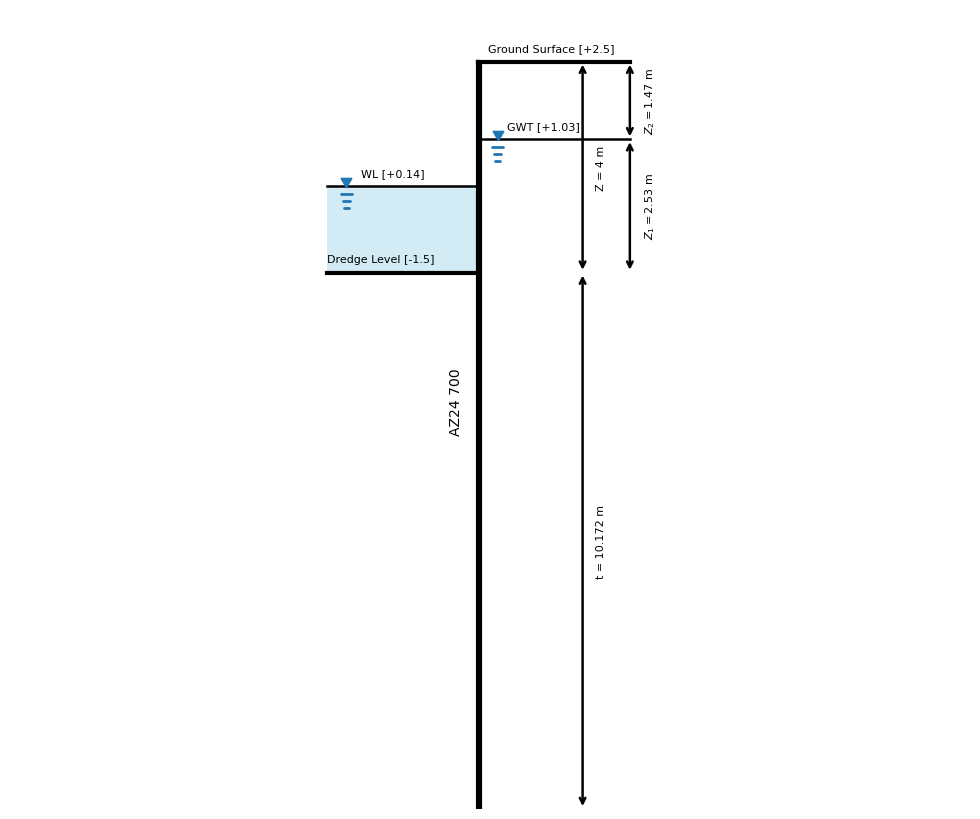
\includegraphics[width=0.90\linewidth]{figures/ch8/final_design.png}
    \caption{2D design cantilever sheet pile}
    \label{fig:final_design}
\end{figure}

\begin{figure}[H]
    \centering
    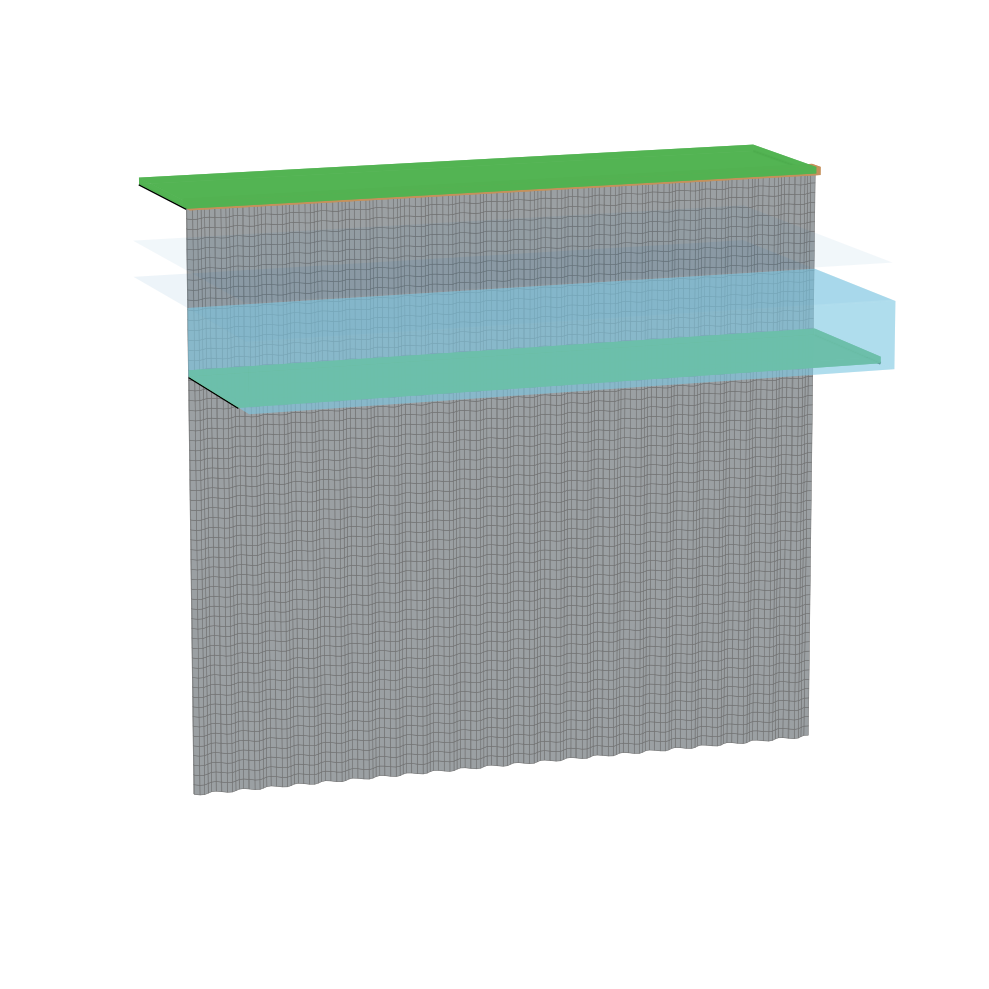
\includegraphics[width=0.70\linewidth]{figures/ch8/3D_final_desgin.png}
    \caption{3D design cantilever sheet pile}
    \label{fig:3D_final_design}
\end{figure}

\newpage
\section{Nature-based solutions}
As stressed in Chapter \ref{chap:sand extraction}, natural damage of the ecosystems occurs on locations where dry sand mines are active. Besides that, in Chapter \ref{chap:hydroanalysis} it was explained that riverbank erosion is a common problem in the Rio Parana Guazu, due to changes of the hydrodynamic parameters of the river. To mitigate these problems, it is the group's intend to use Nature-based solutions.

\subsection{Implementing NbS in this project}
In this section, several NbS will be presented to create a cost-efficient long-lasting, sustainable riverbank. In a first instance, NbS will be explained in detail according to the topics of dry sand mining. Following this, other solutions will be discussed with aim to mitigate the damage done to river banks. Consequently, when it comes to weighing the different NbS against each other this report will make use of the seven goals of the IUCN which must be achieved as good as possible. The seven goals are presented Chapter \ref{chapter:background}, Figure \ref{fig:7g}. Implementations of NbS often face resistance from stakeholders, particularly when these solutions are compared to traditional engineered approaches. From Chapter \ref{chapter:background}, it was made clear why NbS needed to be introduced without a lot of financial constraints. This chapter will work on NbS which are both simple and understandable to all the stakeholders. 


\section{Nature-based solutions for dry sand mining}
%Meer overheidsingrijpen nodig? Zie interview burgemeester: The judiciary forced the government to get involved: do controls, plan and regulate. Now there’s a limit to extract, approx. 2 – 3 m. Before, there wasn’t. En sed de arena report, overheid niet proactief genoeg

%https://www.unep.org/resources/report/sand-and-sustainability-10-strategic-recommendations-avert-crisis
%https://aapepyg.com/2022/11/23/fracking_entre_rios/#_edn4

%While significant strides are taken to implement Nature-based solutions (NbS) against climate change challenges, it is important to note that NbS requires large volume of sand. Additionally, NbS may take time to have the desired effect. Thus in some cases, grey structures (i.e., concrete) may be necessary in the mean time to address challenges in the short- to medium-term. In the context of extreme heat and its impacts on cities, NbS will also be instrumental to promote building designs and materials that require neither concrete infrastructure nor sand (UNEP 2021b). Climate change induced pressures, such as temperature stress and precipitation, will also speed up the degradation of existing infrastructure and the need for upgrading or replacement https://www.unep.org/resources/report/sand-and-sustainability-10-strategic-recommendations-avert-crisis

%Op basis van uitgebreid, door deskundigen beoordeeld bewijsmateriaal concludeerde het Compendium van wetenschappelijke, medische en media-bevindingen die de risico's en schade van fracking aantonen, dat het niet mogelijk is om de techniek van de winning van onconventionele koolwaterstoffen 17Sed de Arena 2023 I Valeria Foglia en de daarmee samenhangende winningsactiviteiten niet mogelijk is zonder dat dit een bedreiging vormt voor de menselijke gezondheid, de lucht, het water, de economische vitaliteit op lange termijn, de biodiversiteit en de seismische en klimatologische stabiliteit. SED DE ARENA

This section seeks to propose and evaluate Nature-based solutions (NbS) that can effectively address the environmental and socio-economic consequences of dry sand mining. The analysis focuses on developing strategies that harness natural processes to restore degraded ecosystems, enhance landscape resilience, and promote sustainable resource management. In order to provide a comprehensive understanding, the potential advantages and limitations of each proposed NbS will be critically examined. Furthermore, this section will delineate the intended implementation framework, outlining the methodological approach and practical steps required to translate these solutions into effective, context-specific interventions.

\subsection{Floodplains}
Floodplains are low-lying areas around rivers that naturally flood during periods of high water discharge. When managed and restored appropriately, these zones play a crucial role in maintaining riverine ecosystem functions and mitigating the adverse impacts of human activities such as sand mining and land degradation.

In the context of dry sand mining, floodplains could be a Nature-Based Solution to counteract the degradation of terrestrial and hydrological systems resulting from excessive sand extraction. Dry sand mining frequently occurs in former floodplain areas or adjacent uplands, where the removal of surface materials disrupts soil structure, alters drainage patterns, and reduces the area’s natural capacity to retain water. Restoring and reactivating floodplains in such landscapes helps to re-establish the natural hydrological connectivity between surface and subsurface systems. This process promotes groundwater recharge, initiate soil sedimentation and mitigates erosion caused by wind and surface runoff. Moreover, re-vegetated floodplains provide new habitats for native species, contributing to the overall ecological recovery of mined areas. As such, floodplain restoration in dry sand mining zones supports landscape resilience, reduces the long-term environmental footprint of extraction activities, and facilitates a more sustainable post-mining land use.

Restored floodplains offer significant opportunities for local community engagement, livelihood diversification, and socio-economic development. Once stabilized and re-vegetated, these areas can be utilized for sustainable land uses such as flood-resilient agriculture, agroforestry, and controlled grazing, which maintain ecological functions while providing income for local populations. Additionally, floodplains can serve as sites for eco-tourism, recreation, and environmental education, fostering a stronger connection between communities and their natural surroundings. The enhancement of biodiversity and landscape aesthetics further increases the cultural and recreational value of these areas. Moreover, the restored floodplain’s role in improving water retention and soil fertility can directly support local food and water security, especially in regions affected by the environmental degradation of dry sand mining. Through community-based stewardship, floodplain restoration can therefore become a catalyst for sustainable rural development and long-term environmental resilience.

\subsection{Metal-tolerant plants}
As mentioned in section \ref{sect:dryminingeffects}, iron concentrations in the ground water have increased by 2200\% since sand mining operations have started. Meanwhile, manganese concentrations are above the recommended concentration limits and polyacrylamide poses a danger to the users' health. Clearly, there is a need for limiting the amount of metal elements and polluters that infiltrate the groundwater.

The use of metal-tolerant plants, such as phytostabilizers and hyperaccumulators, represents an effective Nature-based solution for mitigating contamination and surface runoff in areas affected by dry sand mining. These plant species have the capacity to absorb, immobilize, or stabilize pollutants, including heavy metals and chemical residues from washing processes, within their roots or above-ground tissues. By establishing vegetation on disturbed or contaminated soils, this method reduces the mobility of harmful substances, prevents their leaching into nearby water bodies and the aquifer, and enhances overall soil stability.

In addition to pollutant control, these plants help reduce surface runoff by increasing soil infiltration capacity and root cohesion, thereby minimizing erosion and the spread of sediments. Over time, the vegetative cover contributes to ecosystem recovery, transforming degraded mining landscapes into self-sustaining, biologically active systems.
Within the Paraná Delta, several naturally occurring plant species exhibit tolerance to moderate metal contamination, conditions which can be associated with post-mining sites. Examples include:

\begin{itemize}
    \item Phragmites australis (reed): known for high tolerance to heavy metals and ability to stabilize sediments \autocite{popaHeavyMetalsAccumulation2023}.
    \item Typha domingensis (southern cattail): native to wetlands in a delta; capable of uptaking and accumulating metals \autocite{solimanTyphaDomingensisPers2024}.
    \item Schoenoplectus californicus (California bulrush): efficient in reducing nutrient and contaminant loads in water.
    \item Spartina densiflora (cordgrass): salt- and metal-tolerant grass found along deltas and coastal zones.
\end{itemize}

These species are native or naturalized in the Paraná Delta region and can therefore be used without compromising local biodiversity or ecological integrity \autocite{m.eidPhytoremediationHeavyMetals2020}. 

\subsection{Vegetated buffer zones}
Vegetated buffer zones are strips of land planted with dense vegetation, such as grasses, shrubs, and trees, established between areas of active land use (dry mining sites) and surrounding environments such as settlements, agricultural fields and nature. In the context of dry sand mining, these buffers function as a natural barrier that mitigates the spread of dust, noise, and pollutants generated by extraction activities.

From an ecological perspective, vegetated buffer zones play a vital role in stabilizing soil, reducing wind speed, and capturing airborne particles, thereby improving local air quality and minimizing off-site impacts. The root systems of the plants anchor the sandy substrate, preventing erosion and surface runoff, while the vegetation canopy traps dust and enhances microclimatic conditions by increasing humidity and reducing temperature fluctuations.

In addition to their environmental benefits, buffer zones contribute to biodiversity enhancement by creating transitional habitats that support a variety of species and small fauna. They also serve as visual and acoustic screens, reducing noise and improving the aesthetic quality of the landscape. When designed with native and drought-tolerant species, vegetated buffers require minimal maintenance and can thrive in the disturbed conditions typical of mining landscapes.

Moreover, the establishment of buffer zones can provide socio-economic advantages for local communities through community-based planting initiatives. Overall, vegetated buffer zones represent a cost-effective and multifunctional Nature-Based Solution that simultaneously addresses environmental degradation, air quality concerns, and landscape restoration in areas affected by dry sand mining.

\subsection{Implementation in Ibicuy area}
The area shown in Figure \ref{fig:PAI} includes the Cristamine S.A. sand mine (located an the right down corner) and another sand extraction site located just next to the primary school (Escuela Primaria). These mining activities have a strong influence on the surrounding landscape and local air quality. By changing the orange surrounded area into a floodplain and the blue lines into vegetated buffer zones these influences could be mitigated. 

The restoration approach by involving floodplains could be used between the area of primary school and the Cristamine mine, with the road as its boundary, as a floodplain restoration zone (orange area). This solution would be particularly valuable after mining operations have ended, allowing the area to naturally recover, increase biodiversity, and provide flood protection and water storage capacity.

In the shorter term, the vegetated buffer solution could effectively reduce dust emissions and protect the local community. Establishing dense vegetation, around the primary school would help minimize dust dispersion into the school grounds, improving air quality for the children and teachers.
Similarly, implementing vegetated buffers along the main road would limit dust movement caused by sand transportation, improving air quality, visibility and nuisance for nearby residents and road users.

From an economic feasibility perspective, these solutions are relatively cost-effective compared to large-scale engineering interventions. Vegetated buffers require moderate initial investment in planting and maintenance but offer long-term benefits in ecosystem services, reduced health costs, and improved landscape aesthetics. Floodplain restoration needs a bigger investment amount. This could be funded through mine closure obligations or environmental offsets, making it a sustainable and financially viable option for the area.


\begin{figure}[H]
    \centering
    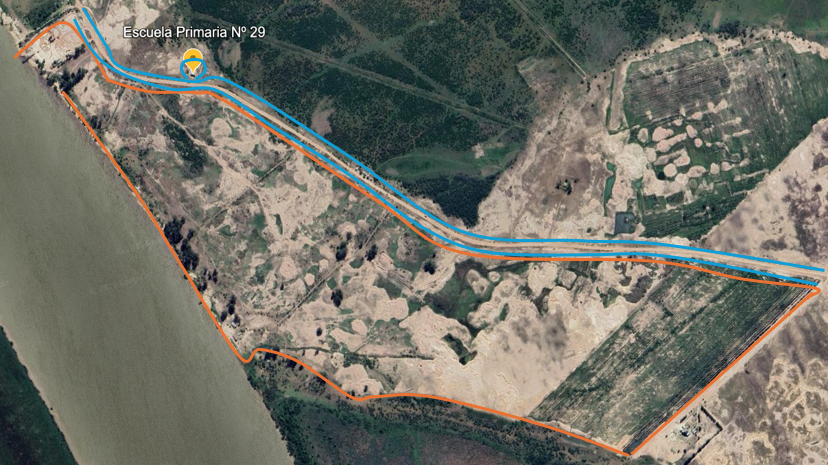
\includegraphics[width=0.75\linewidth]{figures//ch8/omgevingschooltje2.png}
    \caption{Implementation area of possible NbS}
    \label{fig:PAI}
\end{figure}

\section{Nature-based solutions for bank erosion}
Nature-based solutions (NbS) use natural processes and ecosystems to address environmental challenges such as dry sand mining, but also river bank erosion and flood risk. These will be treated in this section. For river bank protection, NbS can include restoring wetlands, planting vegetation, and implementing natural flood management techniques. These solutions not only protect the river banks and infrastructure, but also improve water quality, support wildlife, and create recreational spaces.


\subsection{Natural flood management}
Natural Flood Management (NFM) is a NbS that consists of using natural materials to slow the flow of water through the land and reduce the chance of flash flooding, as well as increasing water storage throughout the landscape \autocite{therivertrust5EasyWays}. Using NFM upstream means that water takes a lot longer to reach lowlands and downstream areas. 

A number of techniques are used in NFM, such as Natural leaky dams. This technique means placing a series of logs across a watercourse mimics the effect of naturally fallen trees. Whilst it’s important not to block the water completely, slowing the flow eases pressure downstream and reduces the risk of flooding, especially after heavy rain. The pathway of the cargo boats found on Marine Traffic is as follows: along the Rio Parana Guazu, leaving out the Rio Ibicuy, and up until Puerto Ibicuy a few times a year. 

Since cargo ships require deep, unobstructed channels, leaky dams are only placed in sites away from the main navigation routes. This ensures they do not interfere with shipping while still providing flood protection downstream. This tells us that in order to adopt this method in the Rio Parana Guazu, the logs will have to be placed above Puerto Ibicuy given that these ships would harm the NbS. 

\subsection{Mangroves}
Another NbS technique used that could the river banks could benefit from are mangroves.
Sand mining in these zones leads to severe loss of soil structure \ref{chap 6: effect and damage on the river bank}. This not only accelerates coastal erosion but also diminishes the capacity of these landscapes to retain water and support biodiversity. Restoring and expanding mangrove forests in degraded coastal and estuarine areas can help reverse these impacts by re-establishing the natural balance between land and water.

Mangroves are fresh and saltwater-tolerant trees and shrubs that are present in intertidal zones, including river deltas and estuaries. Their dense root systems trap sediment, reduce wave energy, and stabilize shorelines, making them an excellent Nature-Based Solution (NBS) for riverbank protection in coastal water environments. There are different types of mangroves that can serve in diverse situations. Planting mangroves and local vegetation along the riverbanks, particularly in areas with shallower edges. Mangroves are highly effective at stabilizing shorelines due to their dense root systems which trap sediments and reduce wave energy, like those from the cargo ships. If the right trees are planted in the right places, a mangrove creation can go a long way towards managing the flow of water through river catchments \autocite{ferreiraPropagulosMangueVermelho2024}. A Figure \ref{fig:Rhizophora mangle} of a Rhizophora mangle (red mangrove) and a Figure \ref{fig:Avicennia germinans} of Avicennia germinans (black mangrove) as well as their specifics are shown below:

\begin{figure}[H]
    \centering
    \begin{subfigure}{0.48\textwidth}
        \centering
        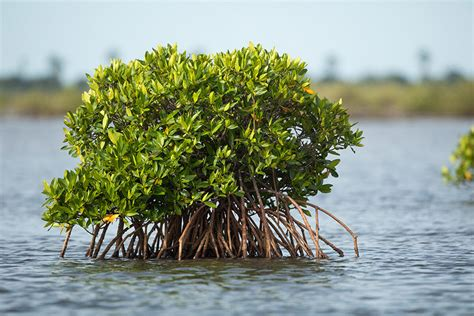
\includegraphics[width=\linewidth]{figures/ch8/mangrove1.jpeg}
        \caption{\textit{Rhizophora mangle} implementation area}
        \label{fig:Rhizophora mangle}
    \end{subfigure}
    \hfill
    \begin{subfigure}{0.48\textwidth}
        \centering
        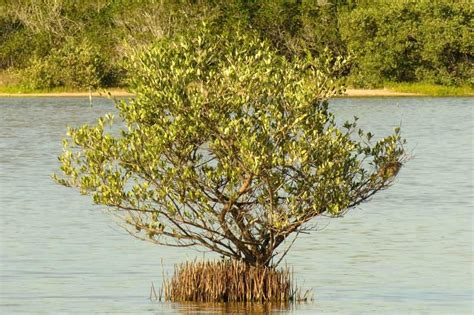
\includegraphics[width=\linewidth]{figures/ch8/mangrove2.jpeg}
        \caption{\textit{Avicennia germinans} implementation area}
        \label{fig:Avicennia germinans}
    \end{subfigure}
    \caption{Implementation areas of possible Nature-based solutions (NbS) using mangroves}
    \label{fig:mangrove_nbs}
\end{figure}


\begin{itemize}
    \item Red Mangrove (Rhizophora mangle): Excellent for shoreline stabilization due to its dense prop roots, which trap sediments and reduce wave energy. Often used in coastal restoration projects to prevent erosion and create fish habitats \autocite{sprungHowLongDoes2021}.
    \item Black Mangrove (Avicennia germinans): Thrives in saltier environments and has specialized "pneumatophores" (breathing roots) that help aerate the soil.Effective for improving soil salinity tolerance and supporting biodiversity in highly saline areas \autocite{hammondWhatBlackMangrove2022}.
\end{itemize}

Putting the idea to the test, the locations where these mangroves would be the most useful would of course be where the bank erosion is the worst. In this case that would be the outside of the river turns of the region of interest. That would include locations like the land of stakeholders such as the owner of the Camping La Blanqueada, Camping El Trebol, Camping Ipona Guazu, or Oasis Guazu.

\subsection{Riparian buffer zone}
Riparian buffer zones are strips of vegetation planted along riverbanks to stabilize soil, filter pollutants, and absorb floodwaters. These zones can include a mix of trees, shrubs, and grasses, which work together to protect the bank from erosion and improve water quality as an extra benefit \autocite{ukforestrystandardCreatingManagingRiparian2024}. The principle is almost the same as for the mangroves, but with different types of vegetation and a bit more in front of the mangrove line. For the riparian buffer zone vegetation, the roots of plants bind the soil, reducing erosion caused by wave action and currents. Vegetation slows overland flow, allowing water to infiltrate the ground and reducing the volume of runoff entering the river \autocite{marshallUnderstandingVitalRole2024}. The added value is that in addition to stability, buffer zones also provide habitat for wildlife and create green corridors for biodiversity \autocite{vagheeiFreshwaterRiparianZones2025}. In Figure \ref{fig:riparian zone}, one can see how one of the local landowners integrated the riparian vegetation zone into his property.

\begin{figure}[H]
    \centering
    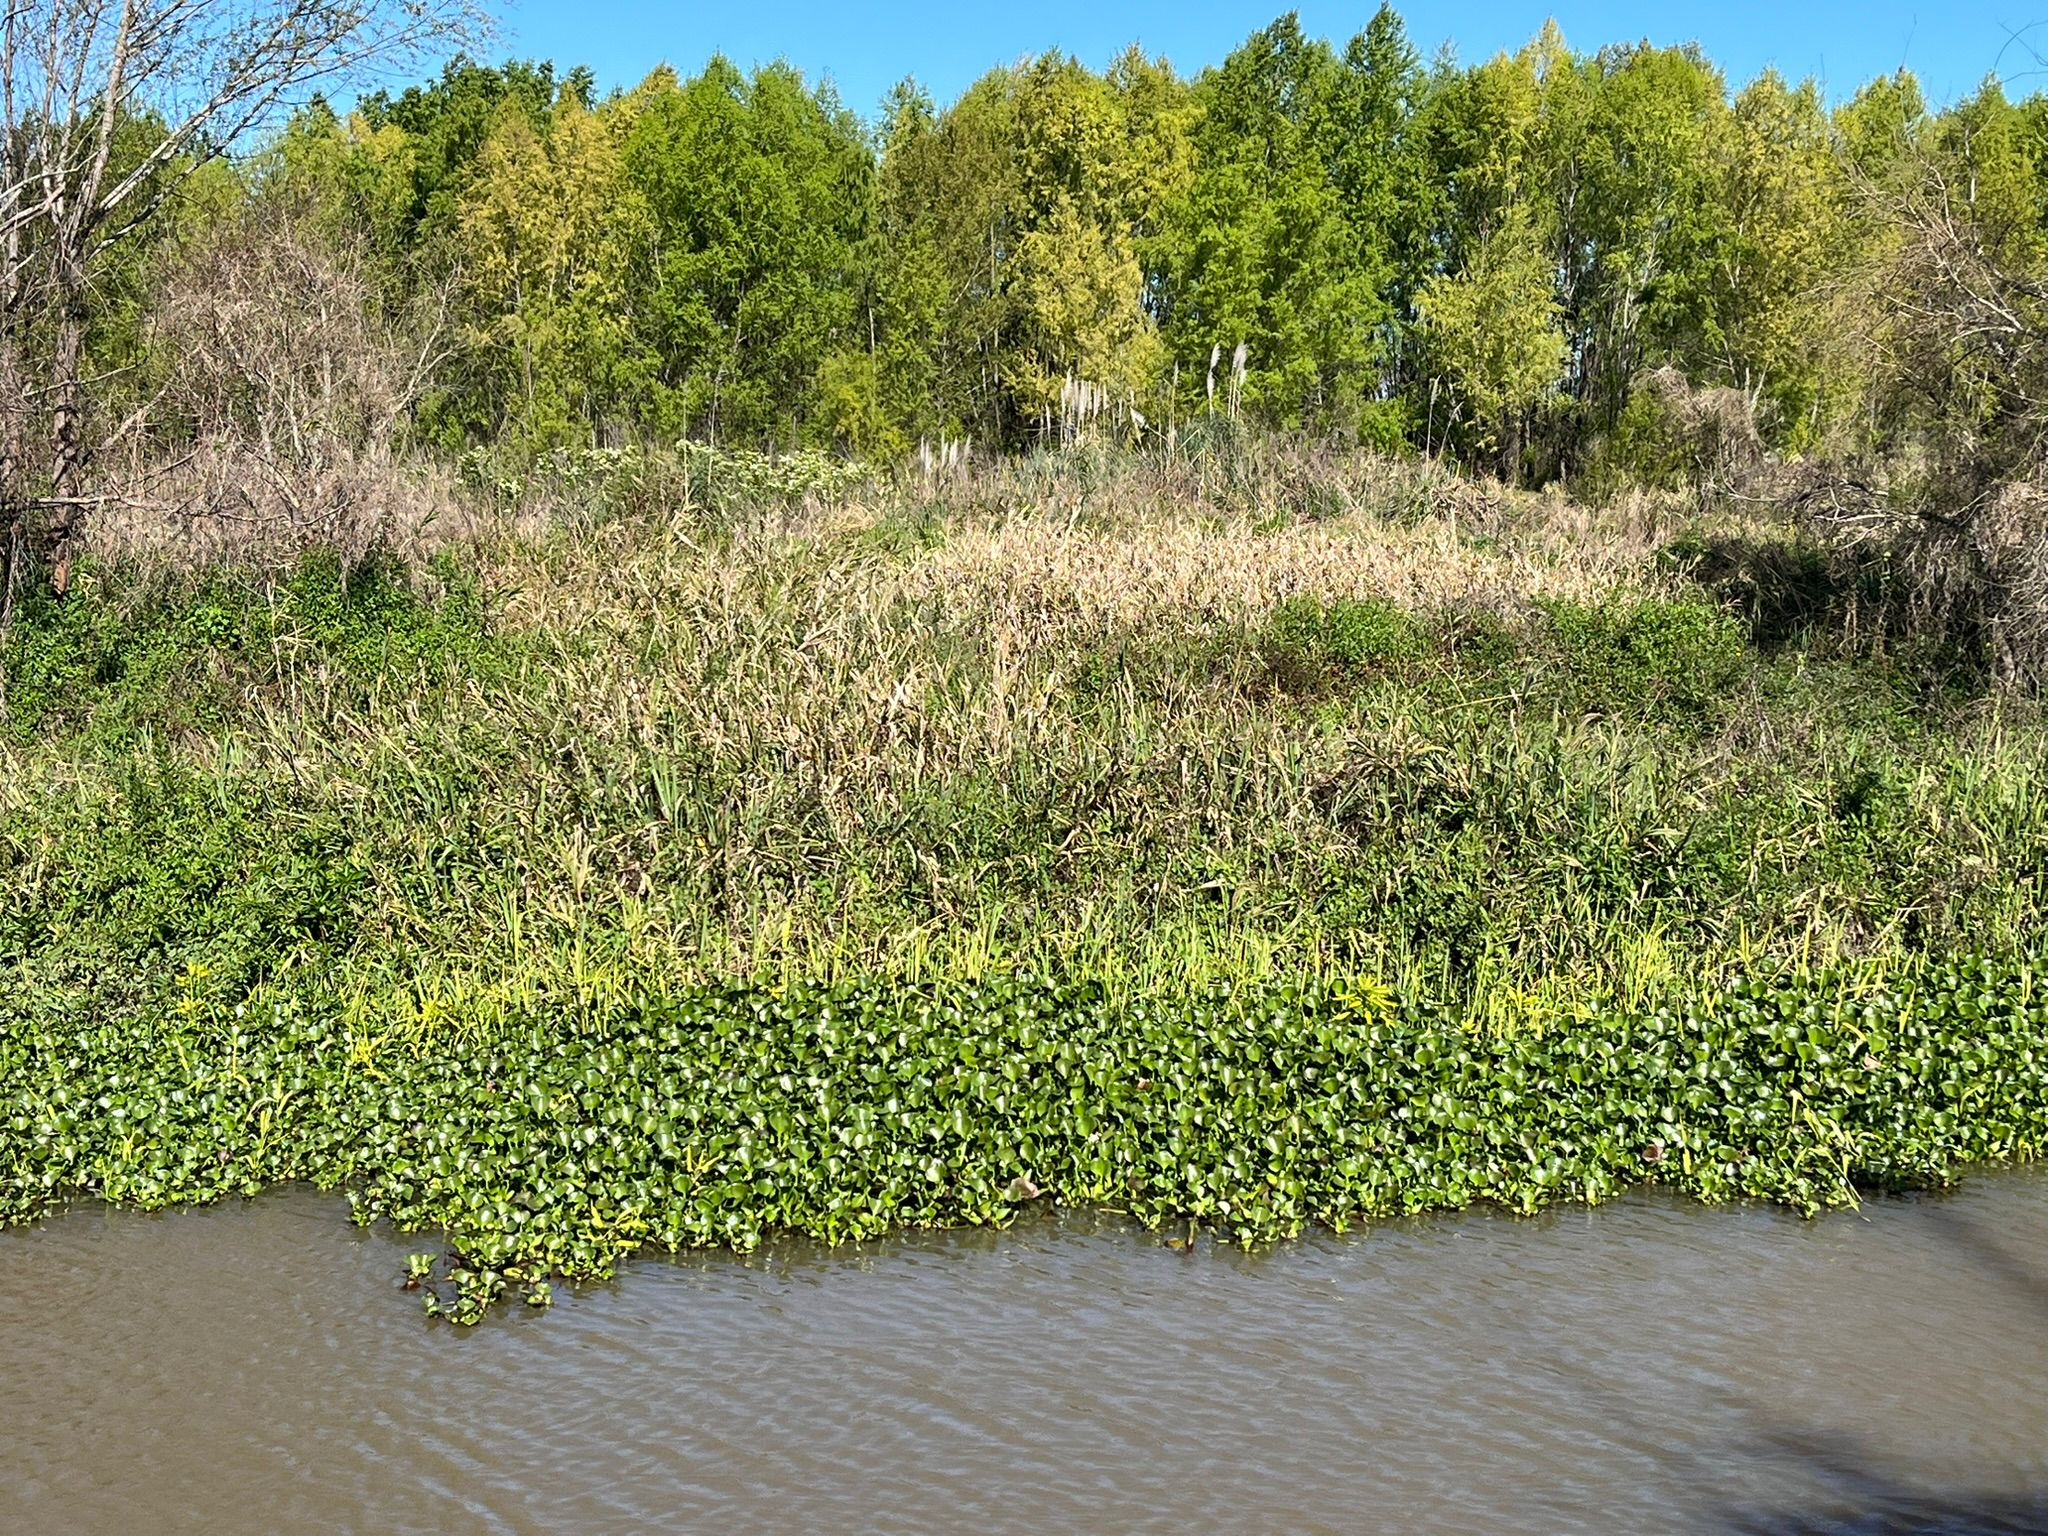
\includegraphics[width=0.5\linewidth]{figures/ch8/riparian.jpg}
    \caption{Riparian buffer zone vegetation}
    \label{fig:riparian zone}
\end{figure}

A list with riparian buffer zone vegetation can be found below:

\begin{itemize}
    \item Willow (Salix humboldtiana): Fast-growing, deep-rooting tree that stabilizes eroding banks, filters pollutants, and provides shade to reduce water temperature \autocite{inaturalistSalixHumboldtiana2020}.
    \item Cockscomb Coral Tree (Erythrina crista-galli): Nitrogen-fixing tree that improves soil fertility, provides habitat for birds and insects, and helps stabilize banks with its root system \autocite{weedsaustraliaCockspurCoralTree2019}.
    \item Inga Tree (Inga uruguensis): Nitrogen-fixing tree that prevents soil erosion, supports pollinators, and provides food for wildlife \autocite{guiadeplantasnativasIngaUraguensisInga2008}.
\end{itemize}


\subsection{Deposited Rock Debris as a NbS}
When visiting Camping Oasis Guazu, the group saw that mitigations strategies had already been tested. The landowner chose to put rocks on the side of the bank to decrease the erosion process as seen in Figure \ref{fig:local solution Camping Oasis Guazu}. These rocks are used to protect the bank from the high tides and wave impacts from the ships passing by.

\begin{figure}[H]
    \centering
    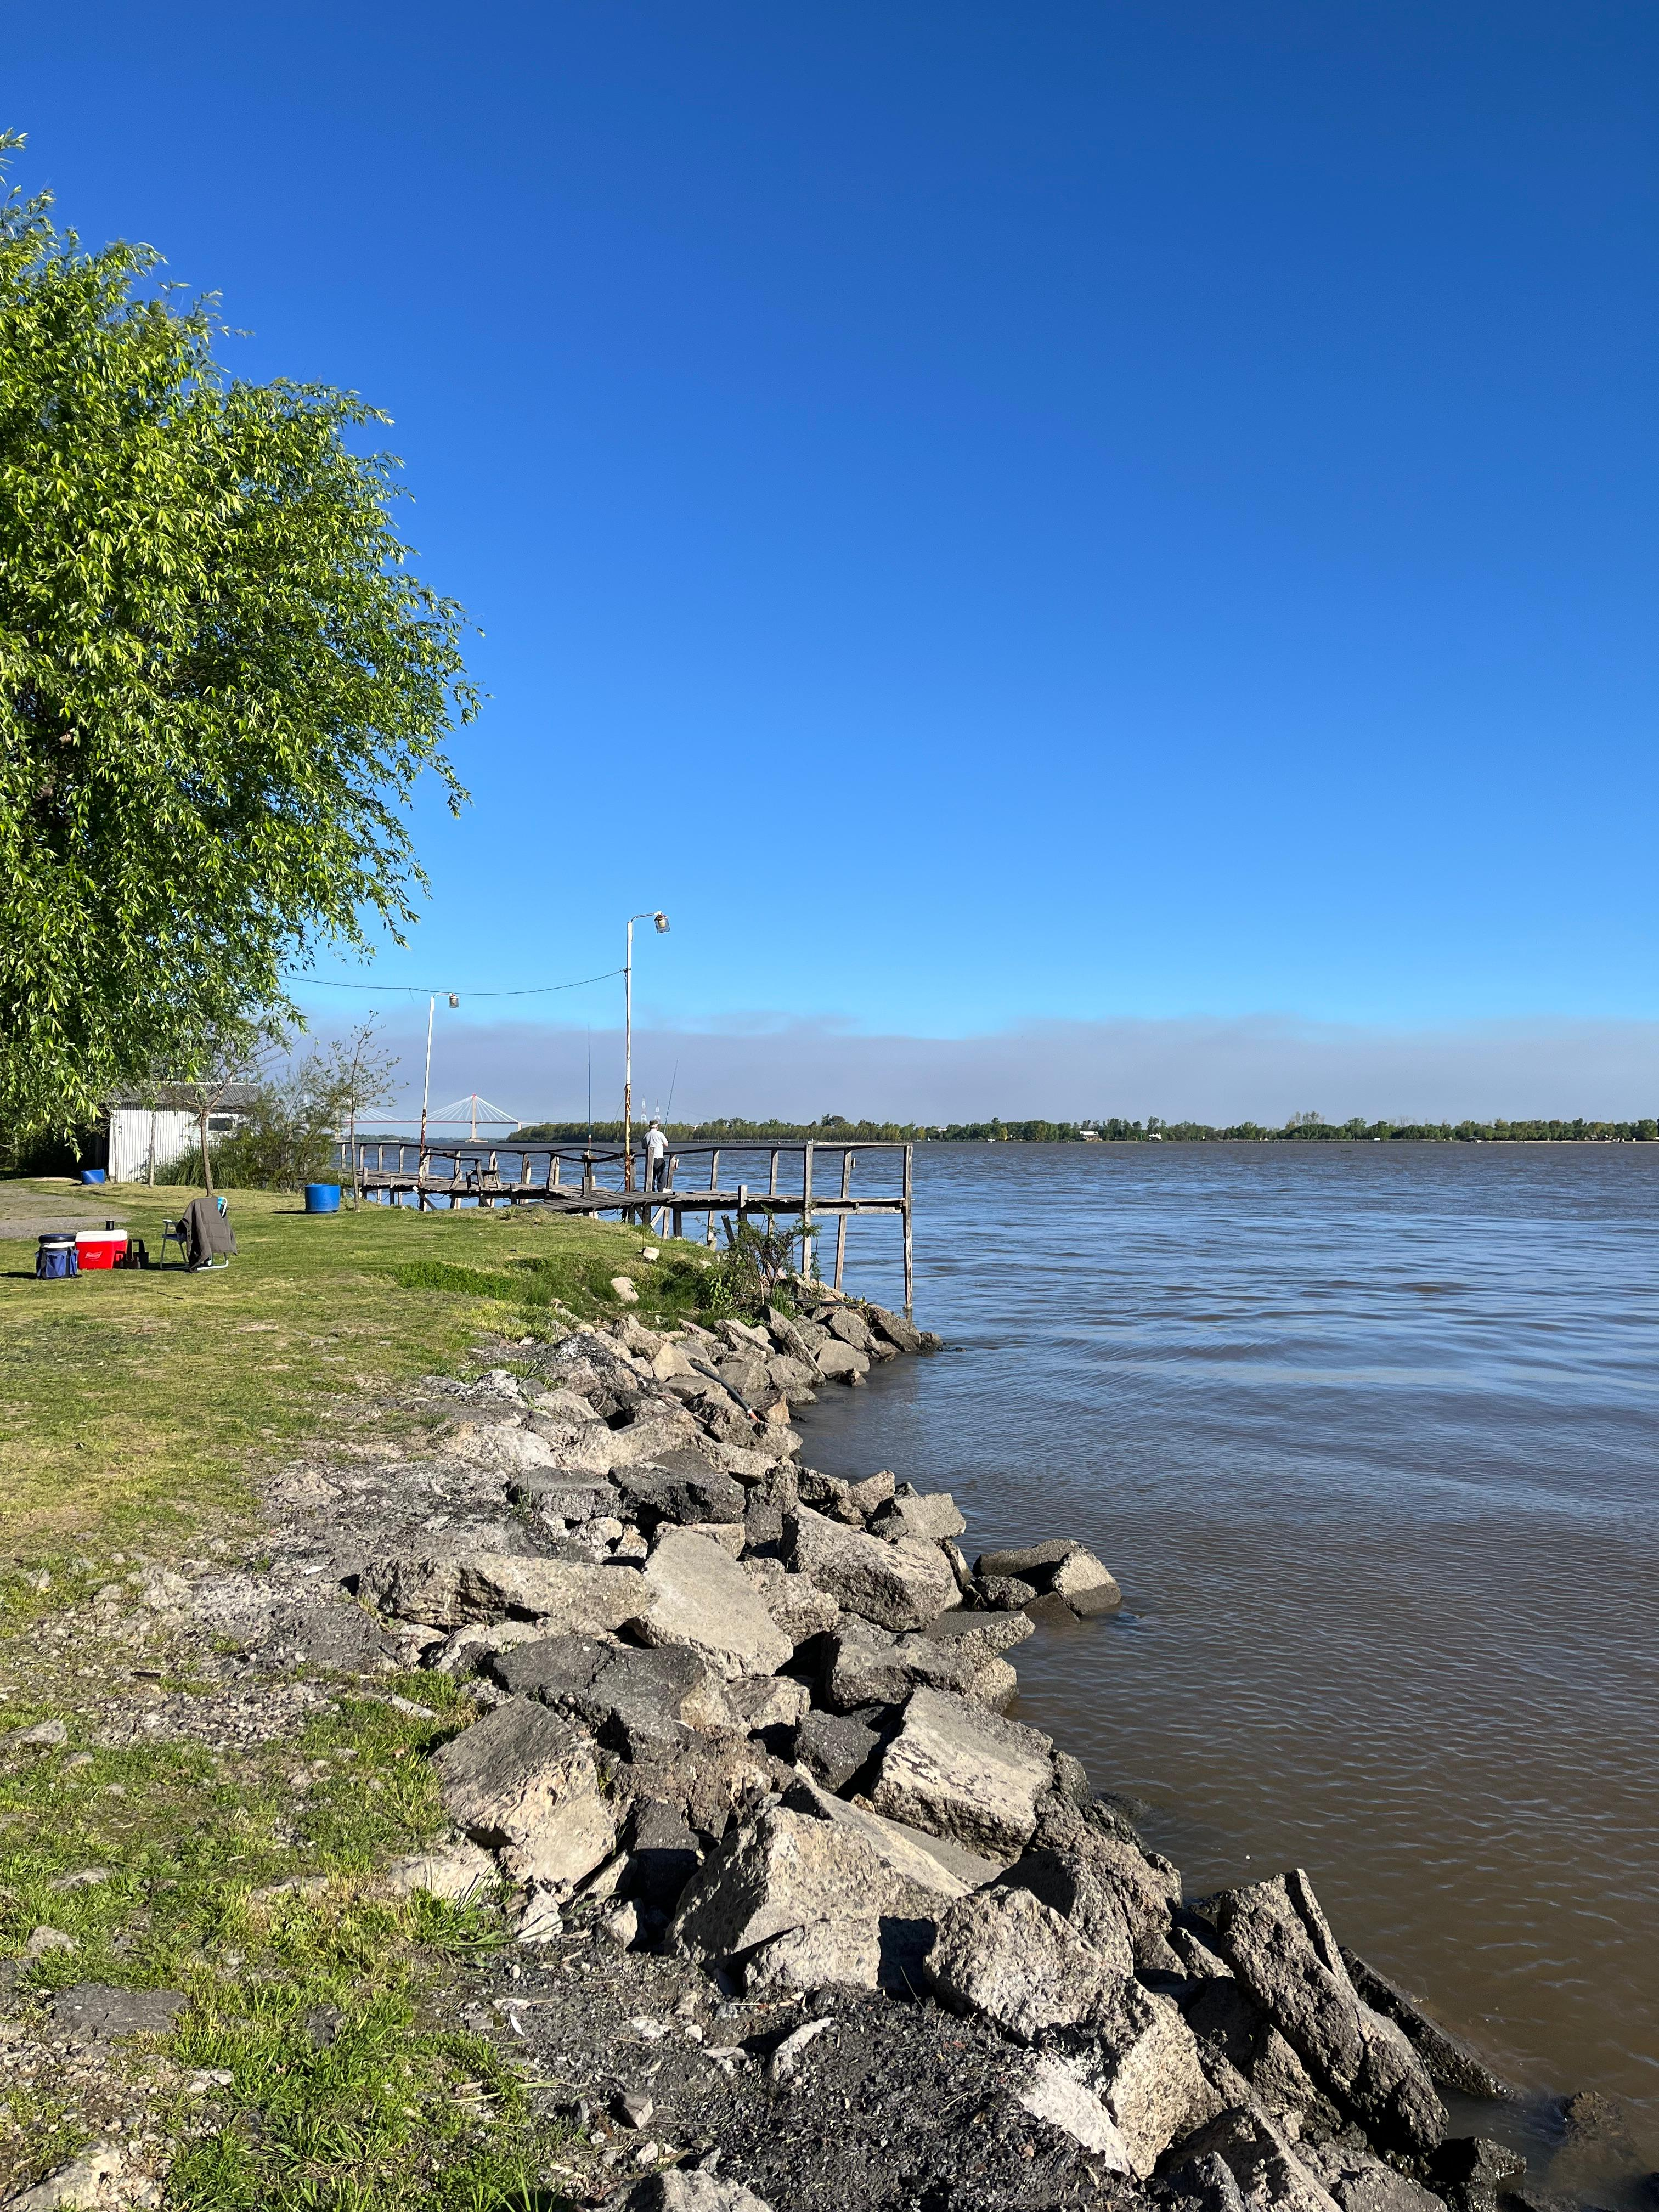
\includegraphics[width=0.5\linewidth]{figures/appendixE/rocks.jpg}
    \caption{Local solution Camping Oasis Guazu}
    \label{fig:local solution Camping Oasis Guazu}
\end{figure}

According to the owner of the land, this solution has significantly contributed to the decrease of land erosion. As this is not a true natural solution, it could not be interpreted as a NbS like this. Nevertheless, incorporating rocks as a buffer for the current, leaving other vegetation more time to take over and contribute to the stability of the banks, that would be a suitable approach to transition towards a 100\% true NbS.






\subsection{Evaluation of the NbS}

The final goal of this Section is to integrate these solutions into the landscape. This could help establish a clearer picture of what can be achieved with these solutions. Table \ref{tab:gradingmatrix} presents the grading of various Nature-based solutions (NbS) according to seven key goals, including climate change mitigation and adaptation, disaster risk reduction, economic and social development, human health, food security, water security, and ecosystem degradation and biodiversity loss. Every NbS is classified on a scale of --, -, 0, +, ++. 

\begin{table}[H]
  \centering
  \caption{Grading by the seven NbS goals}
  \label{tab:gradingmatrix}
  \small
  \renewcommand{\arraystretch}{1.15}
  \setlength{\tabcolsep}{3pt}

  \resizebox{\textwidth}{!}{% zodat hij altijd past
  \begin{tabular}{l
      >{\centering\arraybackslash}p{2.6cm}
      >{\centering\arraybackslash}p{2.4cm}
      >{\centering\arraybackslash}p{2.4cm}
      >{\centering\arraybackslash}p{2.0cm}
      >{\centering\arraybackslash}p{2.0cm}
      >{\centering\arraybackslash}p{2.0cm}
      >{\centering\arraybackslash}p{2.0cm}
      >{\centering\arraybackslash}p{2.0cm}@{}}
    \toprule
    & Climate change mitigation and adaptation
    & Disaster risk reduction
    & Economic and social development
    & Human health
    & Food security
    & Water security
    & Ecosystem degradation and biodiversity loss 
    & Overall grading\\
    \midrule
    Floodplains              & ++ & + & 0  & 0  & + & + & +  & + \\
    Metal-tolerant plants    & 0  & + & +  & ++ & - & + & -  & 0 \\
    Vegetated buffer zones   & +  & 0 & ++ & ++ & 0 & 0 & +  & + \\
    Natural flood management & ++ & + & 0  & -  & 0 & + & 0  & 0 \\
    Mangroves                & 0  & 0 & 0  & 0  & + & 0 & -  & 0 \\
    Riparian buffer zone     & +  & 0 & +  & 0  & + & 0 & +  & + \\
    Rock Debris as NbS       & 0  & 0 & +  & 0  & 0 & 0 & -- & 0 \\
    \bottomrule
  \end{tabular}
  } % einde resizebox
\end{table}

The results of Table \ref{tab:gradingmatrix} show various Nature-based solutions (NbS) across several criteria related to environmental and social benefits. Floodplains show the strongest overall performance, receiving high ratings (++ or +) in most categories, particularly in climate change mitigation, disaster risk reduction and ecosystem protection. Vegetated buffer zones and mangroves also perform well, especially in supporting human health, food security, and biodiversity. In contrast, options like rock debris and metal-tolerant plants provide more focused benefits on one or two topics. Natural flood management demonstrates strong potential in climate adaptation and water security but is more neutral in other areas. These results high-light that while all NbS options contribute to sustainability goals, some provide broader and more integrated ecosystem benefits than others.

